\chapter{Datenauswertung} \label{Datenauswertung}
Die Daten aus Tabellen werte ich nun statistisch aus. Zur Auswertung habe ich \textsf{Jupyter Notebooks} basierend auf Python 3 programmiert. \textsf{Jupyter Notebook} ist eine Open Source Webapplikation. Für das Laden der Daten und zur Auswertung von Lagemaßen wird die Python-Bibliothek \texttt{pandas} verwendet. Für die grafische Darstellung wird die Bibliothek \texttt{matplotlib.pyplot} und für die statistische Auswertung die Bibliothek \texttt{statsmodels} verwendet.

\section{Datenvorverarbeitung}  \label{Datenvorverarbeitung}
Bevor die Daten, in den \textsf{Jupyter Notebooks} ausgewertet werden können, müssen diese zunächst geladen werden. Mit der \texttt{pandas} Bibliothek können die Daten von CSV-Dateien in einen \texttt{Dataframe}, eine zweidimensionale Datenstruktur, geladen werden. Die in Abschnitt \ref{Tabellen} beschriebenen Tabellen lade ich in einzelne \textsf{Notebooks}. Ausnahme bilden nur die Tabellen der Gruppengrößen, die ich alle in ein \textsf{Notebook} lade. Zudem erstelle ich ein zusätzliches \textsf{Notebook}, welches die Tabelle der Fahrgastwechselzeiten lädt, jedoch nur die Beschreibung der Daten enthält. Beim Laden der Dateien wurde ging ich immer auf dieselbe Weise vor:

\begin{lstlisting}[language=Python]
import pandas as pd
file_suffix = ".csv"
 
def load_data(path):
    return pd.DataFrame(pd.read_csv(path+file_suffix, sep=";"))

\end{lstlisting}
Der Parameter \texttt{path} der Funktion \texttt{load\_data} ist dann immer der Pfad zur entsprechenden CSV-Tabelle ohne Dateiendung.

\section{Beschreibung der Daten} \label{Beschreibung der Daten}
In diesem Kapitel beschreibe ich die gesammelten Daten.\\
Die Anteile an aussteigenden, einsteigenden und Platz machenden Personen kann in \figurename \ref{fig:AnteileProzesstypen} betrachtet werden. In den gesammelten Daten beobachtete ich am meisten Aussteiger, mit einem Anteil von 58.99\%. Einen weiteren großen Anteil bilden Einsteiger, die einen Anteil von 39.98\% besitzen. Als letzte Gruppe sind die Platzmacher zu nennen. Auch wenn in den Beobachtungen nur ein Anteil von 1.02 \% zu erkennen ist, werden diese Personen modelliert. Sie stellen einen wichtigen Teil des Prozesses des Fahrgastwechsels dar, da sie einen großen Einfluss auf die Fahrgastwechselzeit haben. Sie müssen zunächst aus- und daraufhin wieder einsteigen, können somit sowohl als Aus- als auch Einsteiger gezählt werden. Wird im Folgenden von Personen, im Bezug auf deren Wechselzeiten, gesprochen, so werden Platzmacher mit dem Faktor 2 gezählt. Das Verhalten Platz machen wurde an 16.07 \% der Türen beobachtet. In 16.07 Prozent der Fälle gibt es also einen Platzmacher.
\begin{figure}[H]
	\centering
		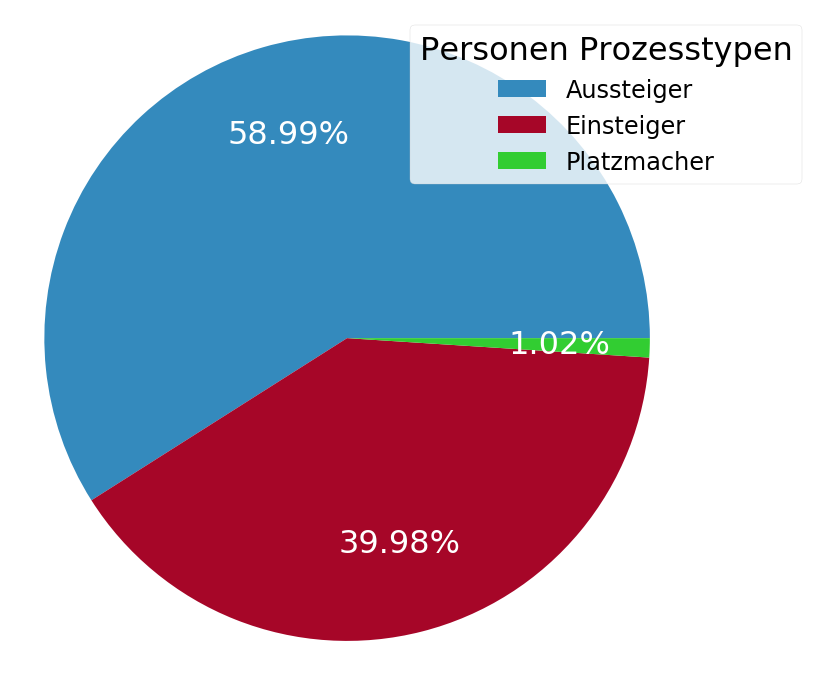
\includegraphics[width=0.6\textwidth]{pictures/data_evaluation/data_description/process_types.png}
	\caption{Anteil der Prozesstypen Aussteiger, Einsteiger und Platzmacher in den gesammelten Daten.}
	\label{fig:AnteileProzesstypen}
\end{figure}
Das Histogramm in \figurename\ref{fig:histAllePersonen} zeigt die Verteilung aller am Fahrgastwechsel teilnehmenden Personen. Hierbei geht es um die Anzahl der Einsteiger, Aussteiger und Platzmacher an jeder Tür.
\begin{figure}[H]
	\centering
		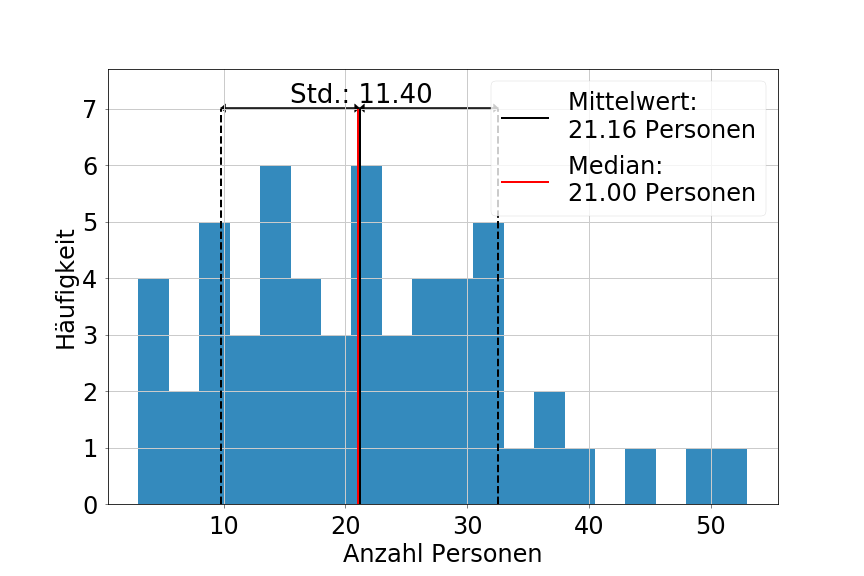
\includegraphics[width=0.7\textwidth]{pictures/data_evaluation/data_description/hist_persons.png}
	\caption{Histogramm der am Fahrgastwechsel beteiligten Personen, mit Später-Ein- und Später-Aussteigern, pro Tür mit einem Mittelwert von 21.16 Personen, einer Standardabweichung von 11.40 Personen und einem Median von 21.00 Personen.}
	\label{fig:histAllePersonen}
\end{figure}
Im Mittel sind es also \ca 21 Personen, die an einer Tür des Zuges ein-, aussteigen oder Platz machen. Auch der Median liegt bei 21 Personen und es besteht eine Standardabweichung von ungefähr 11 Personen.
\section{Fahrgastwechselzeiten} \label{Zeiten}
Mit Hilfe der Tabelle der Fahrgastwechselzeit (Ausschnitt \tablename \ref{tab:times}) beantworte ich nun die Forschungsfrage \ref{item:Fahrgastwechselzeiten} "`Kann die Fahrgastwechselzeit aus der Anzahl der Aus-, Einsteiger und Platzmacher abgeschätzt werden?"'. Um dies zu erreichen, führe ich eine lineare Regression mit der Methode der kleinsten Quadrate durch. Die erklärende Variable $x$ ist die Anzahl der am Prozess beteiligten Personen, und die Zielvariable $y$ ist die Fahrgastwechselzeit in Sekunden. Bevor ich die Regression durchführe, gebe ich zunächst ein Überblick über die Variablen. \cite{Fahrmeir.2009} nennen dies als ersten Schritt der Regressionsanalyse. \\
Für die Wechselzeiten untersuche ich nicht nur die Fahrgastwechselzeit, sondern auch die Kernwechselzeit (siehe \ref{Zeiten Tabelle}). Somit untersuche ich nicht nur den Zusammenhang der Anzahl der Fahrgäste und der Fahrgastwechselzeit, sondern auch der Zusammenhang zwischen der Anzahl der Kern-Personen (ohne Später-Ein- und Später-Aussteiger) und der Kernwechselzeit. Möchte man wissen, wie lange eine gewisse Anzahl an Personen für einen Fahrgastwechsel benötigen, so ist der Zusammenhang zwischen Kernwechselzeit und der Anzahl der Kern-Ein-, Kern-Aussteiger und Platzmacher interessant. Hier fällt der Störfaktor, dass Personen mit gewissem zeitlichem Abstand noch ein- oder aussteigen weg. Die Gesamtheit der Kern-Einsteiger, Kern-Aussteiger und Platzmacher werden im Nachfolgenden mit Kern-Personen bezeichnet, wobei Platzmacher doppelt gezählt werden. Möchte man jedoch betrachten, wie lange ein Zug durchschnittlich im Bahnhof verweilen muss, bis der Fahrgastwechsel beendet ist, ist der Zusammenhang zwischen Fahrgastwechselzeit und Anzahl der am Prozess beteiligten Personen interessanter. Im Nachfolgendem ist zu beachten, dass Platzmacher immer mit Faktor zwei gezählt werden, wenn es um die Wechselzeiten geht, da diese Personen sowohl aus- als auch einsteigen.\\ 
Für den ersten Überblick der Variablen bestimme ich die Lagemaße Mittelwert, Median und Standardabweichung und stelle die Verteilung mit Histogrammen grafisch dar (\cite{Fahrmeir.2009}). Für die Regressionsanalyse zeige ich das Histogramm der Kern-Personen (ohne Später-Ein- und Aussteiger) des Fahrgastwechsels, in \figurename \ref{fig:histPersonen}.
\begin{figure}[H]
	\centering
		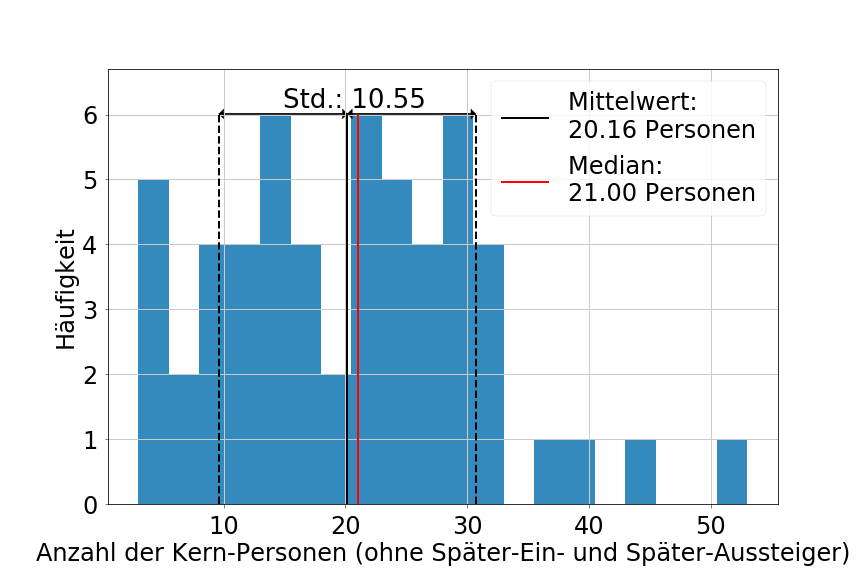
\includegraphics[width=0.7\textwidth]{pictures/data_evaluation/transferTime/hist_core_persons.png}
	\caption{Histogramm der am Fahrgastwechsel beteiligten Kern-Personen (ohne Später-Ein- und Später-Aussteiger) pro Tür mit einem Mittelwert von 20.16 Personen, einer Standardabweichung von 10.55 Personen und einem Median von 21 Personen.}
	\label{fig:histPersonen}
\end{figure}
Die Anzahl der gefilmten am Prozess beteiligten Kern-Personen schwankt zwischen 3 und 53 Personen, wobei die Anzahl der Kern-Personen in den meisten Videos zwischen 9 und 31 Personen liegt. Durchschnittlich sind es \ca 20 (20.16) Personen, die an einer Tür ein-, aussteigen oder Platz machen. Mehr als 32 Kern-Personen kommen in den Daten nur vereinzelt vor, weshalb für eine große Anzahl von Kern-Personen nur eine sehr ungenaue Aussage getroffen werden kann (\cite{Fahrmeir.2009}). Der Median des Datensatzes liegt bei 21 Kern-Personen pro Fahrgastwechsel. Zudem ist anzumerken, dass es sich um eine unsymmetrisch linksseitige Verteilung handelt.

Nicht nur die Kern-Personen der Beobachtungen werden hier betrachtet. Die Kernwechselzeit stelle ich ebenfalls in einem Histogramm dar (siehe \figurename \ref{fig:histTimes}). Hier ist zu erkennen, dass die Kernwechselzeit einen Mittelwert von 18.2 Sekunden besitzen. Der Median liegt hierbei bei 18.0 Sekunden und die Standardabweichung beträgt 8.3 Sekunden. 
\begin{figure}[H]
	\centering
		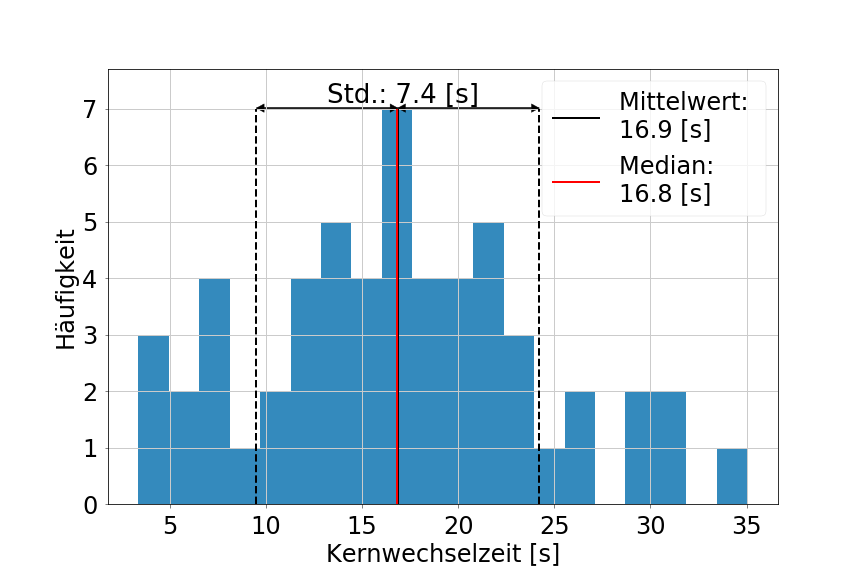
\includegraphics[width=0.7\textwidth]{pictures/data_evaluation/transferTime/hist_core_transfer_time.png}
	\caption{Histogramm der Kernwechselzeit, ohne Später-Ein- und Aussteiger, pro Tür mit einem Mittelwert von 18.2 Sekunden einem Median von 18.0 Sekunden und einer Standardabweichung von 8.3 Sekunden.}
	\label{fig:histTimes}
\end{figure}
Der Wert der benötigten Sekunden liegt zwischen 3.4 und 35.0 Sekunden. Die Verteilung ist hierbei symmetrischer als die der Kern-Personen, kann jedoch auch als eher linksseitig beschrieben werden.

Nachdem nun die Daten für die Kernwechselzeiten und Kern-Personen betrachtet wurden, stelle ich als nächstes die Histogramme für die Fahrgastwechselzeiten und Personen (mit Später-Ein- und Später-Aussteiger) vor. Das Diagramm der Personen ist in \figurename \ref{fig:histAllePersonen} zu sehen. \\
Die Anzahl der am Prozess teilhabenden Personen schwankt, wie bei den Anzahlen bei denen Später-Ein- und Später-Aussteigende nicht beachtet wurden, zwischen 3 und 53 Personen. Der Mittelwert der am Prozess beteiligten Personen erhöht sich durch das Einbeziehen späterer Fahrgäste jedoch von 20 auf \ca 21 (21.16) Personen. In den Daten der Personen liegt die überwiegende Mehrzahl der Anzahl an Fahrgästen zwischen 9 und 32 Personen. Auch hier gibt es wenige Prozesse, bei denen mehr als 32 Personen gezählt wurden. Genaue Aussagen können für diese Anzahlen nicht getroffen werden. Die Verteilung der Personen ist hierbei etwas weniger linksseitig als bei der Verteilung der Kern-Personen, sie ist jedoch auch unsymmetrisch links verteilt.

Nun wird zuletzt die Verteilung der Fahrgastwechselzeit betrachtet. Auch hierfür erstellte ich ein Histogramm, das in \figurename \ref{fig:histAllTimes} betrachtet werden kann.
\begin{figure}[H]
	\centering
	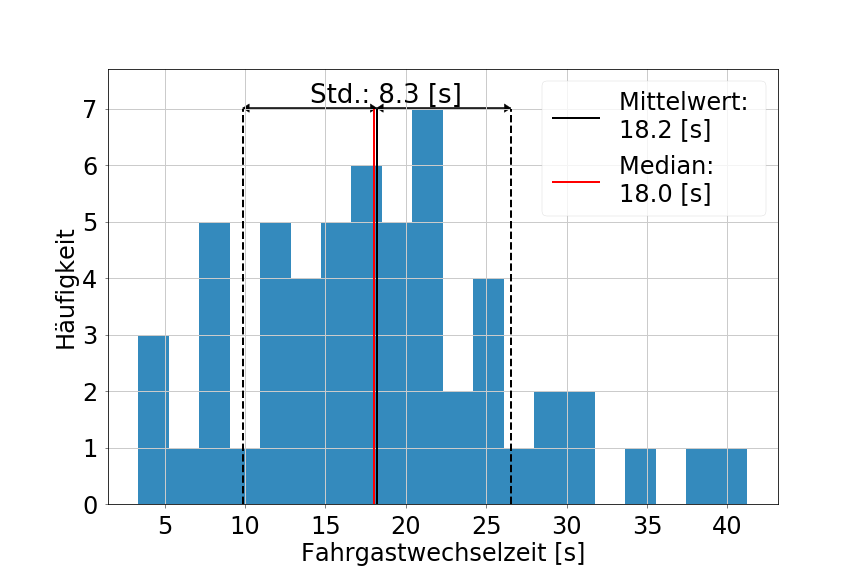
\includegraphics[width=0.7\textwidth]{pictures/data_evaluation/transferTime/hist_transfer_times.png}
	\caption{Histogramm der Fahrgastwechselzeiten pro Tür mit einem Mittelwert von 18.2 Sekunden einem Median von 18.00 Sekunden und einer Standardabweichung von 8.3 Sekunden.}
	\label{fig:histAllTimes}
\end{figure}
Die Werte für die Fahrgastwechselzeiten liegen zwischen 3.4 und 41.2 Sekunden. Für mehr als 32 Sekunden sind hierbei ebenfalls nicht sehr viele Daten gegeben, was auch hier zu Ungenauigkeiten in der Auswertung führen könnte. Die Verteilung ist ebenfalls leicht linksseitig.

Im nächsten Schritt untersuche ich nun der grafische Zusammenhang zwischen der Zielgröße und erklärenden Variable. Dadurch kann "`ein erster Überblick über die Art [...] und Stärke des Zusammenhangs gewonnen werden" (\cite{Fahrmeir.2009}: 13). \\
Zunächst betrachte ich die Kernwechselzeit in Abhängigkeit der Kern-Personenzahl. Wie auf \figurename \ref{fig:zusammenhangsAnalyse} zu erkennen ist, besteht ein annähernd linearer und monoton steigender Zusammenhang zwischen Anzahl der Kern-Personen und Kernwechselzeit. Ebenfalls zu erkennen ist, dass die Streubreite für größere Anzahlen an Kern-Personen sich erhöht.
\begin{figure}[H]
	\centering
		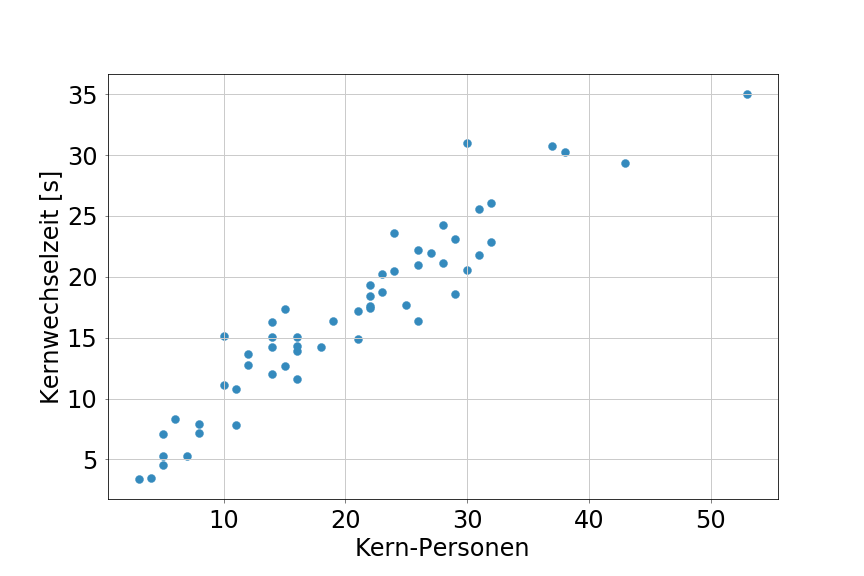
\includegraphics[width=0.7\textwidth]{pictures/data_evaluation/transferTime/core_coherence_analysis.png}
	\caption{Streudiagramm zwischen Anzahl der Kern-Personen (ohne Später-Ein- und Später-Aussteiger), und der Kernwechselzeit in Sekunden. Annähernd linearer und monoton steigender Zusammenhang.}
	\label{fig:zusammenhangsAnalyse}
\end{figure}
Nun stelle ich ebenfalls das Streudiagramm der Fahrgastwechselzeit in Abhängigkeit der Anzahl der Personen dar.
\begin{figure}[H]
	\centering
		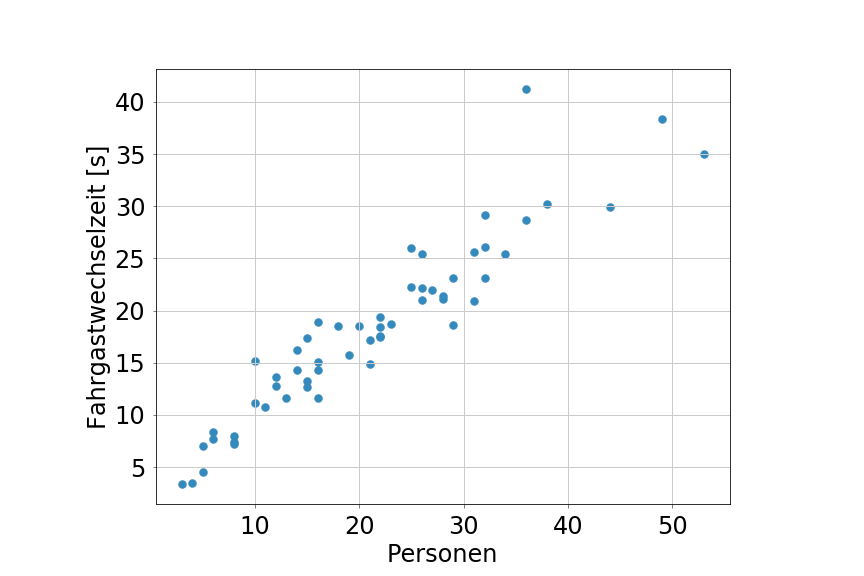
\includegraphics[width=0.7\textwidth]{pictures/data_evaluation/transferTime/coherence_analysis.png}
	\caption{Streudiagramm zwischen Anzahl der Personen, die am Fahrgastwechsel beteiligt sind inklusive Später-Ein- und Später-Aussteiger, und der Fahrgastwechselzeit in Sekunden. Annähernd linearer und monoton steigender Zusammenhang.}
	\label{fig:zusammenhangsAnalyseAlle}
\end{figure}
Auch in diesem Streudiagramm in \figurename \ref{fig:zusammenhangsAnalyseAlle} ist ein annähernd linearer monoton steigender Zusammenhang zu erkennen. Die Streubreite für große Anzahl der Personen ist hier noch höher als bei der Kernwechselzeit ohne Später-Ein- und Später-Aussteiger. 

Sowohl bei der Kernwechselzeit in Abhängigkeit der Kern-Personen als auch bei der Fahrgastwechselzeit in Abhängigkeit der Personen, ist ein linearer Zusammenhang erkennbar. Deshalb führe ich für beide Zusammenhänge jeweils eine lineare Regression durch. Wie schon erwähnt, ist die Zielvariable jeweils die entsprechende Zeit (Fahrgastwechselzeit und Kernwechselzeit) und die Kovariable die entsprechende Anzahl an Personen (mit und ohne Spätere). \\
In Anhang \ref{append:LinReg} wird das Vorgehen zur linearen Regression erläutern.

Um die lineare Regression mit \texttt{Python} durchführen zu können, wird die Bibliothek \texttt{statsmodels.formula.api} verwendet. Mit der \texttt{ols} Methode dieser Bibliothek kann ein Modell erstellt werden, welches dieser mit einem R-Style Formular übergeben wird. Dabei verwendet \texttt{statsmodel} das \texttt{patsy} Packet, welches das Formulare und Daten, in Matrizen umwandelt, die der Modellanpassung dienen. Wendet man auf das Ergebnis der \texttt{ols} Methode dann die \texttt{fit} Methode an, so wird das Modell angepasst und  man erhält man ein \texttt{RegressionResultWrapper} Objekt. In diesem Objekt sind die Ergebnisse der Regression zusammengefasst. \\
Für die lineare Einfachregression wird die Regression folgendermaßen aufgerufen:
\begin{lstlisting}[language=Python]
import statsmodels.formula.api as smf

res_lin = smf.ols(formula="time ~ persons", data=data_time).fit()
\end{lstlisting}
Die Variable \texttt{time} und \texttt{persons} die durch das R-Style Formular übergeben werden sind \texttt{Arrays}. \texttt{Time} enthält die gemessenen Fahrgastwechselzeiten und \texttt{persons} die Anzahlen der Personen, die am Fahrgastwechsel beteiligt sind. Die Variable \texttt{data\_time} ist der \texttt{Dataframe} der Tabelle der Fahrgastwechselzeiten. Das Ergebnis \texttt{res\_lin} ist ein \texttt{RegressionResultWrapper}, der unter anderem die Schätzwerte enthält.

Bei der Zusammenhangsanalyse habe ich festgestellt, dass die Daten, sowohl die mit als auch die ohne Spätere, einen annähernd linearen Zusammenhang besitzen. Deshalb führe ich für die Daten ohne Später-Ein- und Später-Aussteiger nun eine lineare Einfachregression durch.\\
Das Modell für die Zielvariable $Kernwechselzeit$ in Abhängigkeit der Kovariable $Kern\text{-}Personen$ (Einsteiger, Aussteiger und Platzmacher ohne Spätere) ist für die lineare Einfachregression also:
\begin{equation}
Kernwechselzeit_i = \beta_0 + \beta_1 \cdot Kern\text{-}Personen_i + \varepsilon_i
\label{eq:LinFahrgastwechselzeit}
\end{equation} 
Die Methode \texttt{fit()} von \texttt{Python} gibt, unter anderem, für die Funktion \ref{eq:LinFahrgastwechselzeit} die Schätzparameter $\hat{\beta_0}$ und $\hat{\beta_1}$ zurück. In diesem Fall ergibt sich für die lineare Regression: $\hat{f}(Kern\text{-}Personen) = \hat{\beta_0} + \hat{\beta_1} \cdot Kern\text{-}Personen$. Diese kann zur Prognose der $Kernwechselzeit$ verwendet werden.
Die von \texttt{Python} zurückgebenden Schätzwerte sind: $\hat{\beta_0}=3.55$ und $\hat{\beta_1}=0.66$. Das Streudiagramm mit der Schätzfunktion $\hat{f}$ und dem Konfidenzintervall der Funktion kann in \figurename \ref{fig:LinReg} betrachtet werden.
\begin{figure}[H]
	\centering
		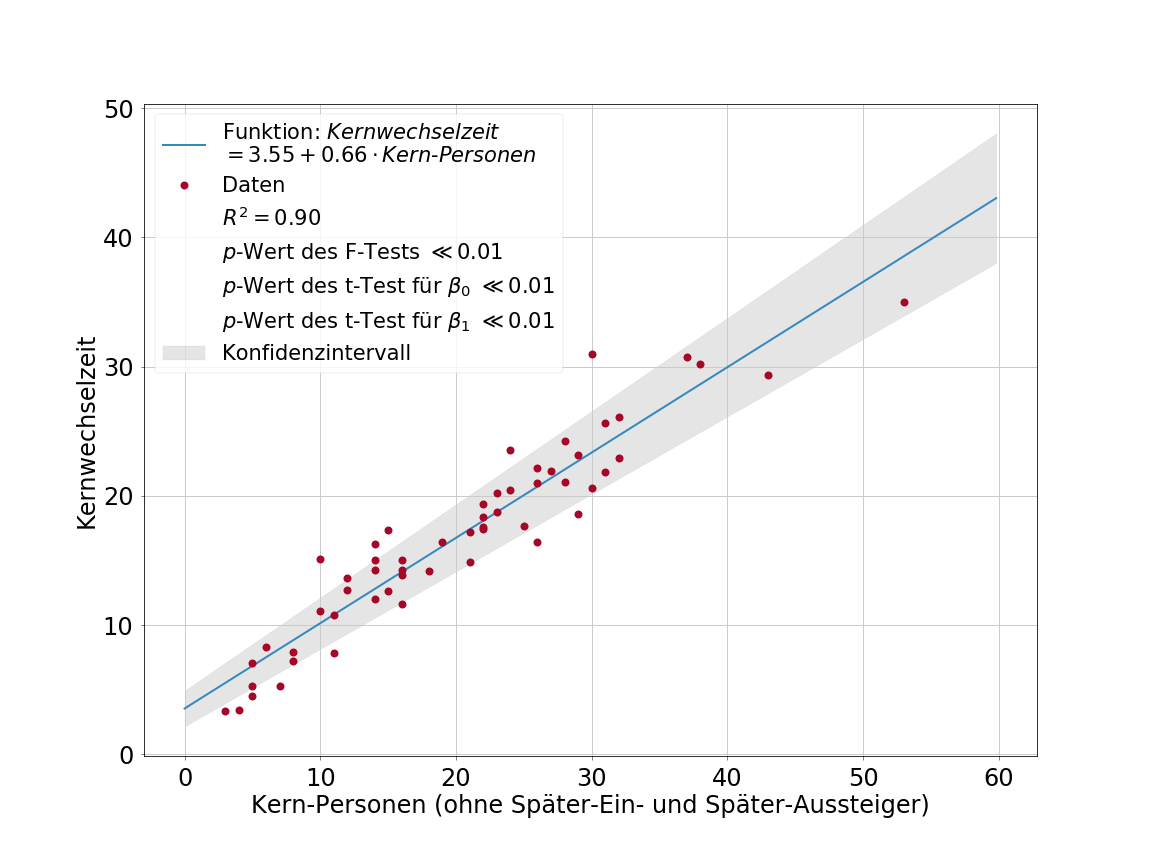
\includegraphics[width=0.7\textwidth]{pictures/data_evaluation/transferTime/lin_core_transfer_time.png}
	\caption{Streudiagramm und lineare Regression der Anzahl der Kern-Personen ($x$) und Kernwechselzeit in Sekunden ($y$) und der geschätzten Funktion: $y = 3.55 + 0.66 \cdot x$, mit dem 95\% Konfidenzintervall.}
	\label{fig:LinReg}
\end{figure}
Nach der Anwendung der linearen Einfachregression überprüfe ich nun, wie gut die Schätzfunktion für die Daten geeignet ist. Dabei ziehe ich das Bestimmtheitsmaß, welches mit $R^2$ bezeichnet wird, heran. Das Bestimmtheitsmaß misst die Güte der Anpassung an die Daten. Auch die Erklärung des Bestimmtheitsmaßes kann im Anhang in \ref{append:rsquared} nachgelesen werden. \\
Die \texttt{fit} Methode gibt das Bestimmtheitsmaß in ihrem Ergebnis zurück. Für die lineare Einfachregression ergibt sich $R^2=0.9$. Dieser Wert liegt somit nah an der 1. Es ist also zu vermuten, dass die Anpassung an die Daten sehr gut ist. 

Es ist jedoch für die Beurteilung des Modells nicht nur wichtig, die Anpassung an die Daten zu betrachten. Zudem führe ich noch statistische Tests durch, um die Regressionsparameter zu überprüfen. "`Voraussetzung für die Konstruktion von (exakten) Tests [...] ist die Gültigkeit der Normalverteilungsannahme der Störgrößen. [Wir setzen] also zunächst unabhängige und identisch verteilte Störgrößen $\varepsilon_i \sim N(0,\sigma^2)$ voraus."'(\cite{Fahrmeir.2009}:111) Die Tests sind jedoch relativ robust gegenüber geringfügigen Abweichungen von der Normalverteilung, weshalb ich im Folgenden annehme, dass die Störgrößen normalverteilt sind (\cite{Fahrmeir.2009}).\\
Im folgenden Abschnitt führe ich nun ein Test auf die Signifikanz der Einflussvariablen durch. Die statistischen Hypothesen für diesen Test lauten:
$$ H_0 : \beta_j = 0 \ \ \text{gegen} \ \ H_1: \beta_j \neq 0. $$
Das betrachtet Testprobleme kann, wenn die Variablen einzeln betrachtet werden, als Spezialfälle des Tests allgemeiner linearer Hypothesen
$$H_0: \boldsymbol{C}\boldsymbol{\beta} = \boldsymbol{d} \ \ \text{gegen} \ \ H_1: \boldsymbol{C}\boldsymbol{\beta} \neq \boldsymbol{d}$$
aufgefasst werden. Wobei $\boldsymbol{C}$ ein $r \times p$ Matrix ist (\cite{Fahrmeir.2009}). Dieser Test wird als F-Test bezeichnet und zeigt die Signifikanz der gesamten Regression an. Die Nullhypothese wäre hier also der Fall, dass alle Schätzparameter, abgesehen von der Konstante, gleich null sind. Die Nullhypothese wird abgelehnt, falls die Teststatistik größer ist als das $(1-\alpha)$-Quantil der entsprechenden F-Verteilung, wobei $\alpha$ das Signifikanzniveau bezeichnet (\cite{Fahrmeir.2009}). Die Definition des Signifikanzniveaus kann im Anhang in \ref{append:Signifikanzniveau} nachgelesen werden. \\
Neben der eben genannten Vorgehensweise, mit dem Vergleich dem kritischen Wert aus der F-Verteilung, gibt es jedoch auch die Möglichkeit, statistische Tests über die sogenannten $p$-Werte durchzuführen. Anstatt die Prüfgröße mit einem bestimmten kritischen Wert zu vergleichen, um über die Ablehnung der Nullhypothese zu entscheiden, vergleicht man den $p$-Wert direkt mit dem vorgegebenen Signifikanzniveau $\alpha$. Der $p$-Wert gibt nämlich gerade die Wahrscheinlichkeit an, unter $H_0$ den beobachteten Prüfgrößenwert zu erhalten. Die Nullhypothese ist also dann zu verwerfen, falls der $p$-Wert kleiner ist als $\alpha$ (\cite{Fahrmeir.2011}).

Das Ergebnis der Regression von \texttt{statsmodel} gibt eben diesen $p$-Wert für die F-Statistik an. Um also zu Testen ob die Schätzgrößen zusammenwirkend Signifikant sind, betrachte ich eben diesen Wert. Zunächst lege ein Signifikanzniveau von $\alpha = 0.01$ fest. Der berechnetet $p$-Wert des F-Test für das Modell der lineare Einfachregression ist $ \ll 0.01$. Die Nullhypothese wird deshalb abgelehnt. Es ist also davon auszugehen, dass die Schätzparameter zusammenwirkend signifikant sind.

Neben der Signifikanz der Regression, teste ich nun auch die Signifikanz der einzelnen Einflussvariablen. Diese Tests werden als t-Tests bezeichnet und besitzen die Hypothesen:
$$ H_0:\beta_j = 0 \ \ \text{gegen} \ \ H_1: \beta_j \neq 0 \ \ j = 0, ..., p$$
Beim einem t-Test ist der kritische Wert für den Ablehnungsbereich der Nullhypothese durch das $(1-\alpha/2)$-Quantil der $t$-Verteilung gegeben.

Auch auf die $p$-Werte der t-Tests kann im Ergebnis von \texttt{Python} zugegriffen werden. Hierbei verwende ich ebenfalls ein Signifikanzniveau von $\alpha = 0.01$. Der $p$-Wert des t-Tests der Konstante ist $\ll 0.01$. Die Nullhypothese kann damit abgelehnt werden, und es kann gesagt werden das der Schätzparameter $\beta_0$ einen signifikanten Einfluss besitzt. Da der F-Test für die lineare Einfachregression dem t-Test des Parameters $\beta_1$ entspricht, und diese für den F-Test schon abgelehnt wurde, kann auch hier gesagt werden, dass die Nullhypothese abgelehnt wird, und der Schätzparameter einen Einfluss auf die Regression besitzt.

Durch die durchgeführten Tests und die Betrachtung des Bestimmtheitsmaß kann angenommen werden, dass das Modell der linearen Einfachregression die Daten sehr gut beschreibt. Da der geschätzte Wert der Kernwechselzeit für 0 Personen jedoch schon bei 3.55 Sekunden liegt, was unplausibel ist, und die Daten mit wenigen Kern-Personen unter der Kurve verbleiben, kam mir die Idee ein Modell anzuwenden, welches sowohl einen logistischen als auch eine linearen Teil enthält.

Dazu führe ich ebenfalls eine lineare Regression mit \texttt{statsmodel} durch. Jedoch ist hier das Modell:
\begin{equation}
Kernwechselzeit = \beta_0 + \beta_1 \cdot \log(Kern\text{-}Personen) + \beta_2 \cdot Kern\text{-}Personen
\end{equation}
Sieht man sich nur das Bestimmtheitsmaß der Regression an, so scheint diese Funktion auch zu den Daten zu passen. Der $R^2$-Wert hat sich für das Modell mit logarithmischem Anteil mit einem Wert von $0.9$ nicht verschlechtert. Auch der $p$-Wert bleibt bei der F-Statistik unverändert $\ll 0.01$. Das Zusammenspiel der Schätzwerte hat also einen Einfluss. Betrachtet man jedoch die $p$-Werte der t-Statistik für die einzelnen Schätzwerte, so wird deutlich, dass die lineare Einfachregression besser für die gegeben Daten geeignet ist, da die $p$-Wert von $\beta_1$ mit $0.02$ und $\beta_0$ mit $0.41$ das Signifikanzniveau überschreiten. Deshalb wird Nullhypothesen für $\beta_1$ und $\beta_0$ angenommen, die Parameter haben höchst wahrscheinlich keinen Einfluss auf die Regression.

Die Fahrgastwechselzeit kann also mit der Funktion 
\begin{equation}
f(Kern\text{-}Personen) = 3.55 + 0.66 \cdot Kern\text{-}Personen
\end{equation}  
durch die Anzahl der am Fahrgastwechsel beteiligten Personen abgeschätzt werden. Damit ist zu sagen das die Kernwechselzeit sich pro Kern-Person um etwa $0.66$ Sekunden erhöht.

Nachdem nun ich die Kernwechselzeit für die beteiligten Kern-Personen ohne Später-Ein- oder Später-Aussteiger mit der linearen Einfachregression geschätzt habe, führe ich nun auch eine lineare Einfachregression für die Fahrgastwechselzeit durch. Hierbei untersuche ich den Zusammenhang zwischen den am Fahrgastwechsel beteiligten Personen, mit Später-Ein- und Später-Aussteigern, als erklärende Variable $x$, und der Fahrgastwechselzeit als Zielvariable $y$. Die Zielvariable gibt dann die Zeit an, welche ein Zug voraussichtlich am Bahnhof verbringen muss, wenn eine bestimmte Anzahl an Personen den Zug verlassen und betreten wollen. Diese Schätzung dient eher der Fahrplan-Planung als die Vorangegangene, welche nur besagte wie lange Personen für einen Fahrgastwechsel benötigen, ohne dabei zu berücksichtigen, dass manche Personen erst später an den Zug gelangen oder aus ihm aussteigen. Das "`später Einsteigen"' und "`später Aussteigen"' Verhalten wird an 35.71 \% der Türen gezeigt.

Auch hier habe ich bei der Zusammenhangsanalyse festgestellt, dass der Zusammenhang annähernd linear ist. Somit führe ich auch hier eine lineare Einfachregression, diesmal mit dem Modell
\begin{equation}
Fahrgastwechselzeit = \beta_0 + \beta_1 \cdot Personen
\end{equation}
durch. Die Variable $Fahrgastwechselzeit$ stellt hierbei die Fahrgastwechselzeit für alle Personen und die Variable $Personen$ die Anzahl der Personen inklusive Späterer dar.
\begin{figure}[H]
	\centering
		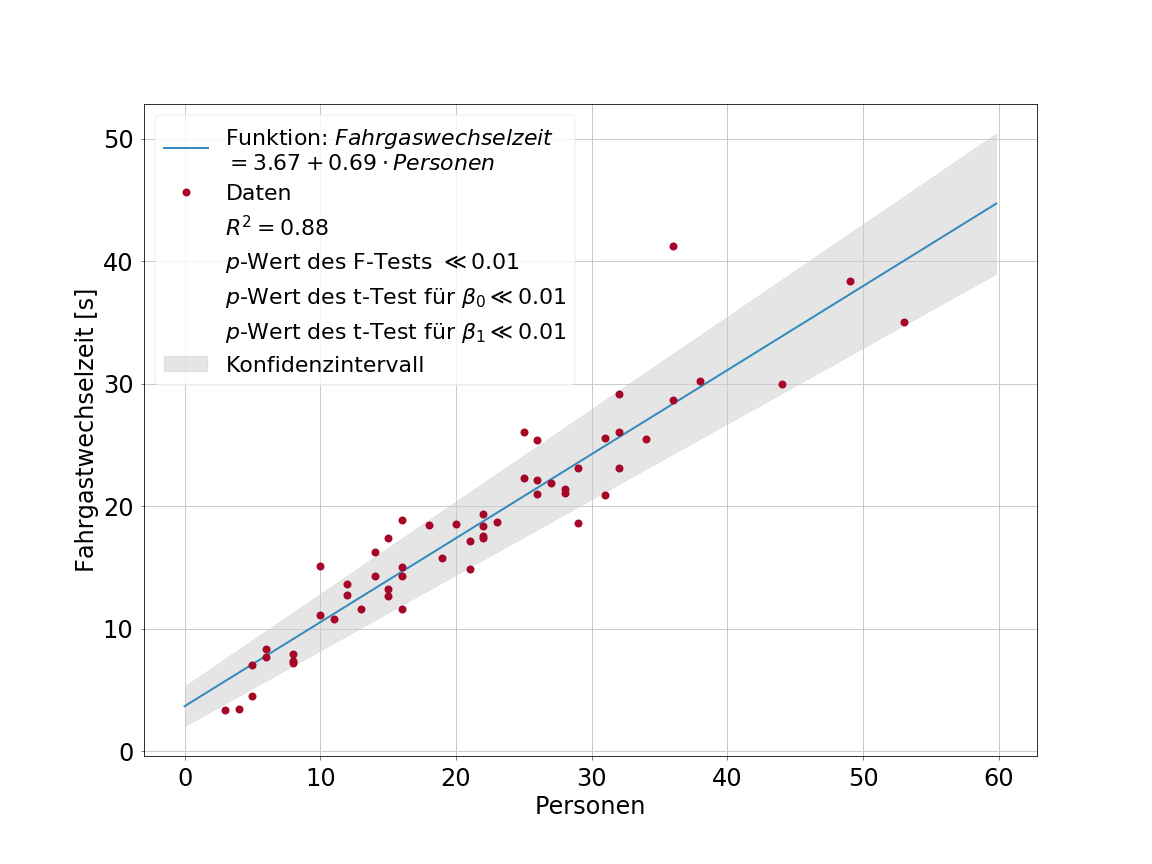
\includegraphics[width=0.7\textwidth]{pictures/data_evaluation/transferTime/lin_transfer_time.png}
	\caption{Lineare Regression zwischen Anzahl der Personen die am Fahrgastwechsel beteiligt sind ($x$) und der Fahrgastwechselzeit in Sekunden ($y$) und der geschätzten Funktion, $y= 3.67 + 0.69 \cdot x$, sowie dem 95\% Konfidenzintervall.}
	\label{fig:LinRegAlle}
\end{figure}
Die von \texttt{Python} zurückgebenden Schätzwerte sind hier: $\hat{\beta_0}=3.67$ und $\hat{\beta_1}=0.69$. Das Streudiagramm mit der Schätzfunktion und dem Konfidenzintervall der Funktion kann in \figurename \ref{fig:LinRegAlle} betrachtet werden.
Die Schätzparameter haben sich hierbei, im Gegensatz zu denen im Modell ohne spätere Personen, also nur etwas erhöht. Die Steigung der Kurve erhöht sich hier von $0.66$ auf $0.69$ und die Konstante der Gerade von $3.55$ auf $3.67$. \\
Das Bestimmtheitsmaß verringerte sich durch die Beachtung der Späteren jedoch auf $0.889$ dieser Wert gibt immer noch eine gute Angepasstheit an die Daten an, zeigt jedoch auch, dass die Schätzung für die Zielgröße wahrscheinlich etwas ungenauer ist als bei der Aussparung der Personen die erst später zum Fahrgastwechsel hinzustoßen. Wie bei der vorangegangenen Untersuchung stimmen auch bei dieser linearen Einfachregression die $p$-Werte für die F-Statistik und die t-Statistik des $\beta_1$ überein, weshalb hier nur die t-Tests durchgeführt werden. Das Signifikanzniveau $\alpha$ besitzt weiterhin den Wert 0.01. Für die Konstante $\beta_0$ ergibt sich für den t-Test ein $p$-Wert der $\ll 0.01$ ist. Die Nullhypothese wird abgelehnt und es kann somit angenommen werden, dass diese Konstante Einfluss besitzt. Auch der $p$-Wert der $\beta_1$ Schätzung ist für den t-Test $\ll 0.01$. Auch hier kann ein Einfluss des Schätzparameters angenommen werden, da die Nullhypothese abgelehnt wurde.

Auch für diesen Zusammenhang versuche ich noch einmal ein Modell mit logarithmischem Anteil anzuwenden. Weil die $p$-Werte der t-Statistik jedoch über dem Signifikanzniveau liegen, wurde auch für die Fahrgastwechselzeit das Modell mit der Geraden angenommen.

Die Funktion 
\begin{equation}
f(Personen) = 3.67 + 0.69 \cdot Personen 
\end{equation}  
kann die Fahrgastwechselzeit also gut abschätzen. Damit ist anzumerken, dass sich die Fahrgastwechselzeit für eine Person mehr um ungefähr 0.69 Sekunden erhöht, und damit nur um 0.03 Sekunden mehr als bei der Kernwechselzeit.

Mit diesen Funktionen können die Wechselzeiten (Kernwechselzeit oder Fahrgastwechselzeit) im Normalfall abgeschätzt werden. Somit kann die Forschungsfrage \ref{item:Fahrgastwechselzeiten} mit Ja beantwortet werden. Mit den Funktionen kann sowohl die wahrscheinliche Zeit für den Fahrgastwechsel als auch die benötigte Haltezeit der U-Bahn, im Standardfall, abgeschätzt werden. Dies Abschätzungen könnten in die Planung von U-Bahn-Stationen und Fahrplänen einfließen. Ein weiterer Verwendungszweck könnte das Einsetzen dieser Funktion bei der Modellvalidierung sein. Wird ein Modell basierend auf dem Entscheidungsprozess erstellt und simuliert, könnten die durch Simulationen erhobenen Fahrgastwechselzeiten mit diesen Funktionen verglichen, und so eine Aussage über die Plausibilität des Modells gemacht werden. Die Ergebnisse können zudem für die Kalibrierung des Modells verwendet werden. 

Die Auswertungen der Fahrgastwechselzeiten mit \textsf{Jupyter Notebook} können im Zusatzmaterial in der Datei \texttt{TransferTime.ipynb} betrachtet werden.
\section{Gruppen} \label{Gruppen}
Im Simulationsprogramm der Firma accu:rate existiert bereits ein Modell für Gruppenverhalten. Da das Verhalten von Gruppen eine Simulation beeinflusst, beschreibe ich in diesem Abschnitt die Auswertung der Gruppentabellen (\tablename \ref{tab:groupsAS}, \tablename \ref{tab:groupsES} und \tablename \ref{tab:groupsPM}). Durch die Auswertung dieser Tabellen beantworte ich die Forschungsfrage \ref{item:Goupsize} "`Kann aus dem Filmmaterial gewonnen werden, welche Gruppengrößen im Fahrgastwechsel auftreten und wie viel Prozent der Personen sich in einer Gruppe mit einer bestimmten Größe befinden?"'.

In der Software von accu:rate werden in einer Tabelle, die in einer Simulation vorkommenden Gruppengrößen, mit dem zugehörigen prozentualen Anteil der Agenten, welche in einer Gruppe dieser Größe sind, angegeben. Deshalb stelle die beobachteten Anteile von Personen in den Gruppen durch ein Kuchendiagramm (\figurename \ref{fig:AnteileGruppen}) dar.
\begin{figure}[H]
	\centering
		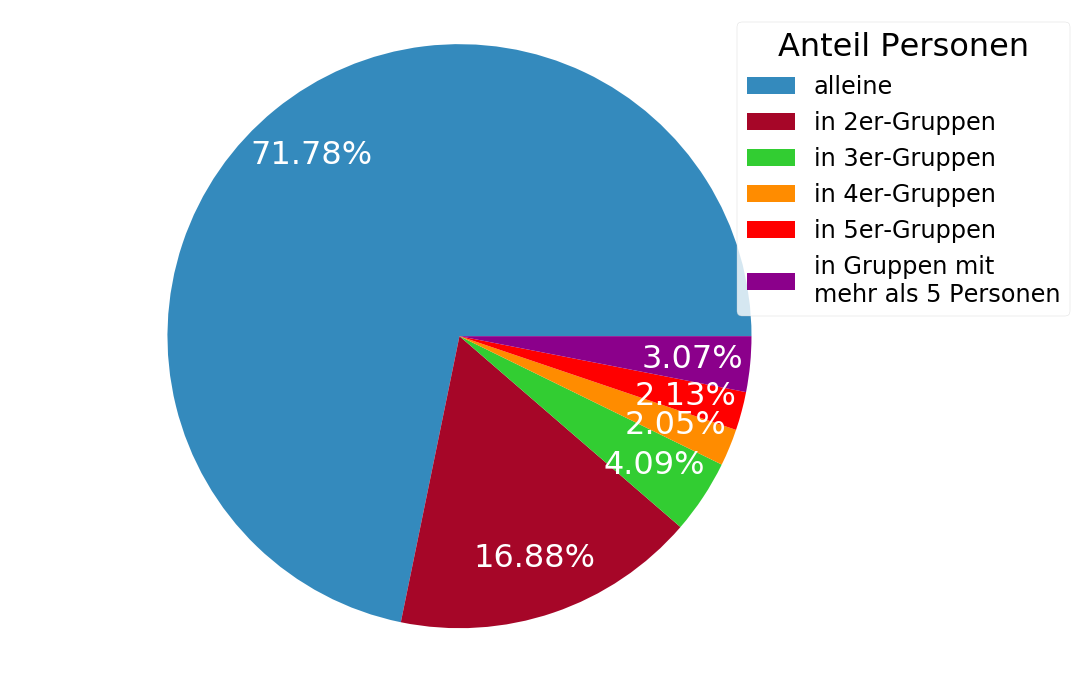
\includegraphics[width=0.7\textwidth]{pictures/data_evaluation/groups/groups.png}
	\caption{Kuchendiagramm der Anteile der Personen, die in einer Gruppe mit einer gewissen Gruppengröße beobachtet wurden.}
	\label{fig:AnteileGruppen}
\end{figure}
Gruppen erkenne ich durch Verhaltensweisen, wie das Sprechen mit oder warten auf andere Mitglieder der Gruppe. Bei den prozentualen Anteilen unterscheide ich nicht zwischen den Prozesstypen Einsteigern, Aussteigern und Platzmachern, da der Prozesstyp keine Auswirkung darauf hat, welcher Gruppengröße eine Person angehört. Da in den Tabellen nur die Anzahl der Gruppe mit einer gewissen Größe in einem Video angegeben ist und nicht die Anzahl der Personen in dieser Gruppe, wurde für die Auswertung die Gruppenstärke mit der Anzahl der vorkommenden Gruppen multipliziert. 

Die meisten beobachteten Fahrgäste sind alleine unterwegs. In dieser Art von "`Gruppe"' ist ein Anteil 71.78\%. Der nächstgrößere Anteil an Fahrgästen befindet sich, mit einem Anteil von 16.88\%, in Gruppen von zwei Personen. Gruppen mit drei Personen machen einen Anteil von 4.09\% aus. 4-er und 5-er Gruppen besitzen nur noch einen Anteil von \ca 2\% (2.05\% für 4-er-, 2.13\% für 5-er-Gruppen).Der letzte in der Grafik aufgeführte Anteil, ist der Anteil der Personen die in Gruppen mit einer Gruppenstärke von mehr als 5 Personen sind. Diese Bezeichnung führte ich ein, da im Filmmaterial zwar Gruppen mit mehr als 5 Personen erkennbar sind, es jedoch schwierig ist, eine allgemein geltende Behauptung zu deren Gruppengrößen und Anteilen anzustellen. So filmte ich \zB eine Gruppe von 11 Personen, es gibt für diese Größe jedoch nur eine einzige Gruppe, die von mir entdeckt wurde. Zudem beobachtete ich keine 10-er, 9-er oder 8-er Gruppen. Es ist jedoch zu vermuten, dass im realen Leben auch Gruppen mit einer Größe von 8, 9, 10 oder mehr als 11 Personen vorkommen. Deshalb wähle ich den Ausdruck von mehr als 5 Personen, da bei einem größeren Datensatz hier wahrscheinlich noch andere Gruppenstärken auftreten. Diese Art der "`Gruppe"' besitzt einen Anteil von 3.07\%.

Die gesammelten Daten geben einen groben Überblick über die unterschiedlichen Gruppenstärken. Die Forschungsfrage, "`Kann aus dem Filmmaterial gewonnen werden, welche Gruppengrößen im Fahrgastwechsel auftreten und wie viel Prozent der Personen sich in einer Gruppe mit einer bestimmten Größe befinden?"', würde ich jedoch nicht mit Ja beantworten. Wie ich beschrieben habe, ist nicht klar, ob mit den gesammelten Daten alle Gruppengrößen des realen Lebens beobachtet wurden. Zudem können die Daten so nicht in das Modell von accu:rate eingefügt werden. Das Modell von accu:rate möchte alle auftretenden Gruppengrößen und deren genauen Prozentualen Anteil. Für einzelne Personen, sowie 2-er und 3-er Gruppen können die Aussagen noch getroffen werden. Bei Personen, die in einer Gruppe von mehr als 5 Personen sind, kann dies jedoch nicht mehr gewährleistet werden. Wenn die Auswertung meiner Beobachtungen in das Modell mit einfließen sollen, müsste dieses angepasst werden. Es müsste die Möglichkeit geben eine Gruppenstärke anzugeben, die beschreibt, dass es sich um eine Gruppe handelt, die aus mehr als 5 Personen bestehen. Die Gruppenstärke könnte dann zufällig gewählt werden. Ein weiteres Problem mit diesen Daten ist, dass argumentiert werden könnte, dass nicht alle Gruppen erkannt wurden. Ich stimme diesem Argument zu. Ich behaupte jedoch, dass alle relevanten Gruppen erkannt wurden. Relevante Gruppen sind für mich Gruppen, die Gruppenverhalten zeigen.

Die Auswertung der Gruppen mit \textsf{Jupyter Notebook} kann im Zusatzmaterial in der Datei \textsl{GroupSize.ipynb} gefunden werden.
\section{Verhaltensweisen und Merkmale} \label{Verhalten}
Nach den Gruppengrößen und Wechselzeiten untersuche ich nun auch die Verhaltensweisen und Merkmale der beobachteten Personen. Dabei werte ich die bereits beschriebene Tabelle der Verhaltensweisen und Merkmale, \tablename \ref{tab:Vehalten}, aus. Durch dieses Vorgehen beantworte ich die Forschungsfragen \ref{item:Verhalten,Verhalten} "`Beeinflussen die Verhaltensweisen "`früher Einsteigen"' und "`Im Weg Stehen"' die Fahrgastwechselzeiten?"' und \ref{item:Vehalten,Merkmale} "`Beeinflussen die Merkmale "`sperrig"', "`langsam"' und "`abgelenkt"' der Fahrgäste die Fahrgastwechselzeit?"'. Bevor ich darauf eingehe, ob und wie sich diese Merkmale und Verhaltensweisen auf die Fahrgastwechselzeit auswirken, betrachte ich zunächst, wie oft diese beobachtet wurden. Ich gehe so vor, um einschätzen zu können, ob die Verhaltensweisen und Merkmale überhaupt relevant sind. Beobachte ich diese nur in sehr wenigen Fällen, so sind sie für die Modellierung uninteressant. Zu diesem Zweck erstelle ich ein Balkendiagramm, welches in \figurename \ref{fig:BalkenVerhalten} zu sehen ist. Die Balken stellen hierbei den prozentualen Anteil der Türen da, an denen das entsprechende Verhalten oder Merkmal gezeigt wurde.
\begin{figure}[H]
	\centering
		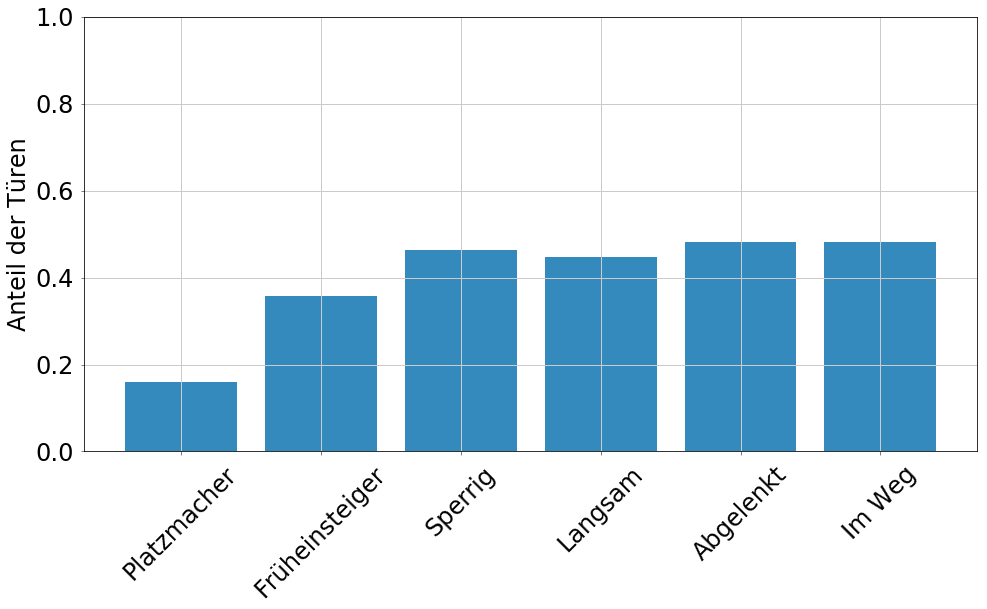
\includegraphics[width=0.8\textwidth]{pictures/data_evaluation/behavior/counts_behavoirs.png}
	\caption{Balkendiagramm der prozentualen Anteile von Verhaltensweisen und Merkmalen. Der prozentuale Anteil bezieht sich hierbei auf den Anteil der gefilmten Türen, an denen das entsprechende Verhalten oder Merkmal beobachtet wurde.}
	\label{fig:BalkenVerhalten}
\end{figure}
Zu erkennen ist, dass alle Verhaltensweisen und Merkmale in weniger als 50 \% der Videos gezeigt wurden. Abgesehen vom Verhalten "`Platz machen"' liegen diese jedoch alle knapp unter oder über 40 \%. Ein Verhalten, welches an \ca 40 \% der Türen gezeigt wird, ist meinem Empfinden nach relevant und sollte, falls es ebenfalls einen Einfluss auf die Fahrgastwechselzeit besitzt, modelliert werden. Um eine Entscheidung, darüber zu treffen ob die Verhaltensweisen "`früher Einsteigen"' und "`im Weg Stehen"', sowie die Merkmale "`sperrig"', "`langsam"' und "`abgelenkt"' für das Modell relevant sind, wird ihr Einfluss auf die Zeit untersucht. Zunächst soll jedoch noch auf die Verhaltensweise "`Platz machen"' eingegangen werden. Platzmacher treten nur an 16.07 \% der Türen auf und liegen damit deutlich unter 40 \%. Wie jedoch schon erwähnt stellen sie einen wichtigen Teil des Fahrgastwechsels dar, da sie sowohl ein- als auch aussteigen müssen, um Platz zu machen. Dass diese Verhaltensweise nur selten auftritt, ist zudem damit zu erklären, dass Platzmacher erst notwendig werden, wenn viele Personen im Wagon sind \bzw am Fahrgastwechsel beteiligt sind. Sind nur wenige Personen im Wagon und somit nur wenig Aussteiger vorhanden, können Fahrgäste ungehindert aussteigen und Platzmacher werden nicht benötigt. Ob es einen Zusammenhang zwischen der Anzahl der Aussteiger und dem Auftreten von Platzmachern gibt, untersuche ich nach der Untersuchung des zeitlichen Einflusses der andere Verhaltensweisen und Merkmale.

Um die Unterschiede der Fahrgastwechselzeit für die genannten Verhaltensweisen und Merkmale zu überprüfen, verwende ich die Fahrgastwechselzeit pro Person. Durch die Verwendung der Fahrgastwechselzeit pro Person wird verhindert, dass die Zeit des Fahrgastwechsels für eine großen Anzahl von Fahrgästen mit der für eine kleinen Anzahl von Personen verglichen wird. Um die Fahrgastwechselzeit pro Person zu gewinnen, erhob ich jedoch nicht die Zeit für jede Person in einem Video. Diese Zeit berechne ich, indem ich die Fahrgastwechselzeit durch die Anzahl der am Fahrgastwechsel beteiligten Personen (mit doppelt gezählten Platzmachern) teile. \\
Durch die Verwendung der Fahrgastwechselzeit pro Person kann das Runden der Zeit auf eine Nachkommastelle jedoch nicht mehr gewährleistet werden. Da eine einzelne Person für den Fahrgastwechsel meist weniger als eine Sekunde benötigt, würde das Runden bei der Fahrgastwechselzeit für eine Person dazu führen, dass ein Vergleich der Zeiten kaum noch möglich ist. Beim Vergleich würde eine Veränderung der Wechselzeit pro Person nicht mehr auffallen, weil die Zahlen durch die Rundung gleich erscheinen. Deshalb runde ich im Nachfolgenden auf 3 Stellen nach dem Komma. Das ist zulässig, da ich die Zahlen nicht weiterverwende, sondern diese nur dem Vergleich der Zeiten dienen. Es muss jedoch vorsichtig mit den Ergebnissen umgegangen werden, weshalb eine zeitliche Veränderung nur dann als relevant angesehen wird, wenn diese Veränderung so erwartet wurde. \\
Um den Vergleich noch etwas besser zu gestalten, habe ich zudem betrachtet, für welche Anzahlen an Personen ich das Verhalten und die Merkmale am häufigsten beobachtet habe. Die Fahrgastwechselzeiten vergleiche ich dann nur in diesem Bereich. Dieses Vorgehen verhindert zum einen, dass ich viele Daten, in denen das Verhalten nicht gezeigt wird, mit wenigen Daten vergleiche, in das Verhalten gezeigt wird. Zum anderen haben habe ich bei der Prognose der Fahrgastwechselzeiten, in Abschnitt \ref{Zeiten}, festgestellt, dass sich die Fahrgastwechselzeit für eine Person mehr nicht um den Faktor 1, sondern 0.66 erhöht. Durch den Vergleich eines gewissen Bereichs wird also auch verhindert, dass die Fahrgastwechselzeit pro Person mit wenig Beteiligte mit der, mit vielen Beteiligten verglichen wird. 

Um den zeitlichen Einfluss der Verhaltensweisen und Merkmale zu untersuchen habe ich Box-Plots verwendet. In einem Box-Plot erstreckt sich die Box immer vom unteren bis zum oberen Quartil der Daten. Der Median wird durch eine Linie in der Box markiert. Die Äußeren Linien (eng.: "`whiskers"') erstrecken sich über den Bereich der Daten, während die äußeren Punkte Ausreißer kennzeichnen. Das untere Quartil bezeichnet das 25\%-Quantil der Daten, während das obere Quartil das 75\%-Quantil darstellt. Als $p$-Quantil wird jeder Wert $x_p$ bezeichnet, für den mindestens ein Anteil $p$ der Daten kleiner oder gleich $x_p$ und mindestens ein Anteil $1-p$ größer oder gleich $x_p$ ist. Somit liegen 75\% der Werte über dem unteren Quartil und 75\% der Werte unter dem oberen Quartil. Der Median ist zudem das 50\%-Quantil der Daten. Abgesehen von der grafischen Betrachtung vergleiche ich zudem die Quantile für die Zeiten. In folgenden Grafiken vergleiche ich immer zwei Box-Plots miteinander. Einer der Box-Plots in den Grafiken entsteht immer aus den Fahrgastwechselzeit von Filmen in denen das Verhalten \bzw das Merkmal nicht gezeigt wurde, der andere die Fahrgastwechselzeit für Türen, bei denen das zu untersuchende Verhalten oder Merkmal vorkam.

Zunächst untersuche ich den Einfluss von Personen, welche das Merkmal "`langsam"' tragen. Hierfür untersuchte ich die Fahrgastwechselzeiten pro Person für Videos mit einer Anzahl von 10 bis 16 Personen.
\begin{figure}[H]
	\centering
		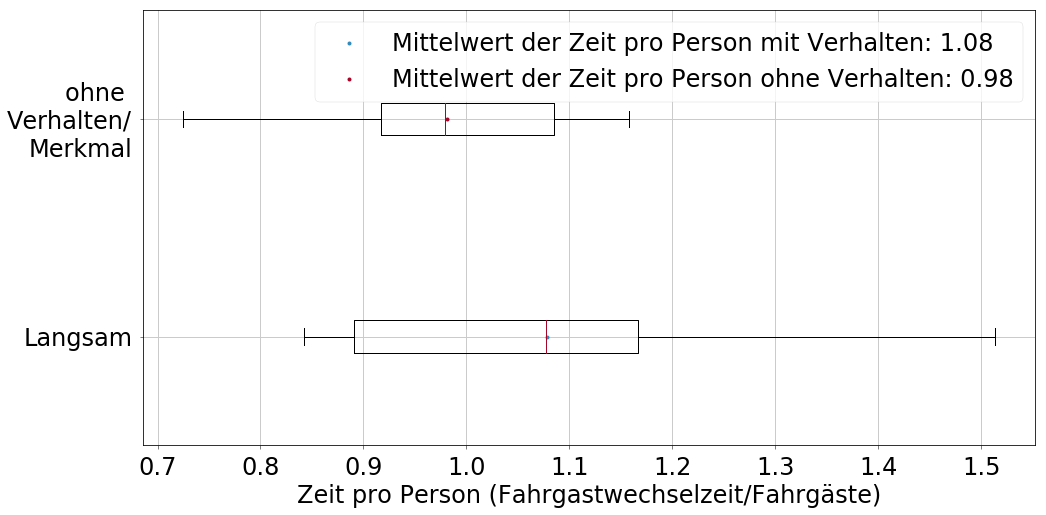
\includegraphics[width=0.8\textwidth]{pictures/data_evaluation/behavior/comp_Langsam.png}
	\caption{Box-Plot für den Vergleich der Zeiten pro Person für Personen die langsam sind und für Personen ohne das Merkmal "`langsam"'.}
	\label{fig:BoxPlotLangsam}
\end{figure}
Wie auf \figurename \ref{fig:BoxPlotLangsam} zu sehen ist hat sich die Fahrgastwechselzeit pro Personen durch langsame Personen im Fahrgastwechsel erhöht. Zu erkennen ist dies durch die Rechtsverschiebung des Box-Plots und dem erhöhten Mittelwert. Ob diese Erhöhung der Zeit signifikant ist, und das Merkmal damit in das Modell aufgenommen werden soll, wird durch den Vergleich von Quantilen entschieden. Zu diesem Zweck verglich ich den Median der Zeit pro Person, mit diesem Merkmal, mit dem oberen Quartil der Zeit pro Person, ohne das Merkmal. Dadurch wird gewährleistet, dass (weniger als) 25\% der Fahrgastwechselzeiten pro Person langsamer waren als das 50\% Quantil der Fahrgäste mit diesem Merkmal. Ist dies gegeben gehe ich davon aus, dass die Auswirkung des Merkmales auf die Zeit signifikant ist und dieses modelliert werden sollte.\\
Der Median der Zeit pro Person für die Fahrgastwechsel in denen "`langsame"' Personen vorkamen liegt bei 1.078 Sekunden. Das obere Quartil für Fahrgastwechsel ohne langsame Personen liegt jedoch bei 1.086 Sekunden. Auch wenn das Quartil der Daten ohne "`Langsame"' nur leicht den Median der Zeiten mit diesen überschreitet, scheint das Merkmal "`langsam"' keinen signifikanten Einfluss auf die gesamten Fahrgastwechselzeiten zu besitzen. Das Merkmal "`langsam"' einer Person wird somit nicht in das Modell mit aufgenommen.

Als nächstes untersuche ich die Auswirkung des Merkmals "`sperrig"'. Hierbei betrachtete ich die Fahrgastwechselzeiten von Videos, in denen zwischen 20 und 27 Personen gefilmt wurden. Auch hierbei ist auf dem Box-Plot, \figurename \ref{fig:BoxPlotSperrig}, zu erkennen das sich die Fahrgastwechselzeit pro Person durch das Merkmal erhöht hat. Während der Mittelwert der Zeiten ohne Sperrige noch bei 0.812 Sekunden lag, liegt er bei den Daten die Personen mit diesem Merkmal bei 0.871 Sekunden.
\begin{figure}[H]
	\centering
		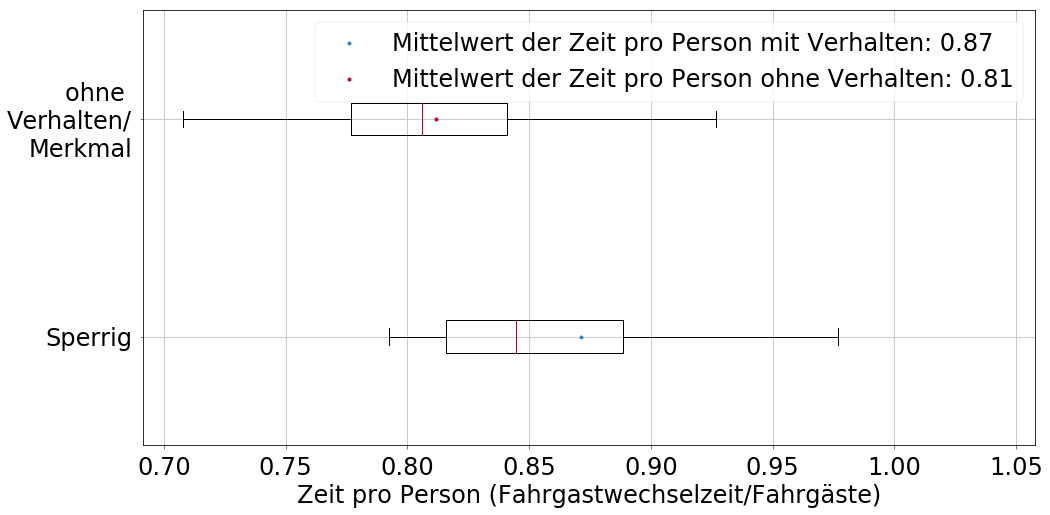
\includegraphics[width=0.8\textwidth]{pictures/data_evaluation/behavior/comp_Sperrig.png}
	\caption{Box-Plot für den Vergleich der Zeiten pro Person für Fahrgastwechsel in denen Personen sperrig sind mit Fahrgastwechsel ohne diese Personen.}
	\label{fig:BoxPlotSperrig}
\end{figure}
Bei diesem Merkmal liegt das obere Quartil der Zeit pro Person, für Personen ohne das Merkmal, bei 0.841 Sekunden, während der Median der Daten mit sperrigen Personen bei 0.844 Sekunden liegt. Da der Median für Personen mit dem Merkmal über dem oberen Quartil der Zeiten ohne dieses liegt, kann gesagt werden, dass der Unterschied signifikant ist. Zudem vermutete ich vor dem genaueren Betrachten, dass das Merkmal "`sperrig"' den Fahrgastwechsel verlangsamen könnte. Durch sperrige Personen kann es passieren, dass nicht mehr, wie im Normalfall, zwei Personen gleichzeitig durch die Tür gehen können, sondern nacheinander Aussteigen müssen, was zu einer Verlangsamung des Prozesses führen könnte. Da der zeitliche Einfluss des Merkmals erklärt werden kann und die Bedingung für die Quantile der Daten erfüllt ist, wird angenommen, dass das Merkmal "`sperrig"' signifikant ist und in das Modell aufgenommen werden sollte.

Als letztes Merkmal untersuche ich nun noch das Merkmal "`abgelenkt"'. Beim Vergleich handelt verwende ich die Fahrgastwechselzeiten für eine Anzahl von 13 bis 21 Personen. Auch für abgelenkte Personen hat sich die Fahrgastwechselzeit pro Person scheinbar erhöht. Es ist jedoch schon deutlich auf dem Bild, \figurename \ref{fig:BoxPlotAbgelenkt}, zu erkennen, dass das 75\%-Quantil der Zeiten für Personen ohne Abgelenkte nicht mehr unter dem Median der Zeiten für Fahrgastwechsel mit diesen liegt.
\begin{figure}[H]
	\centering
		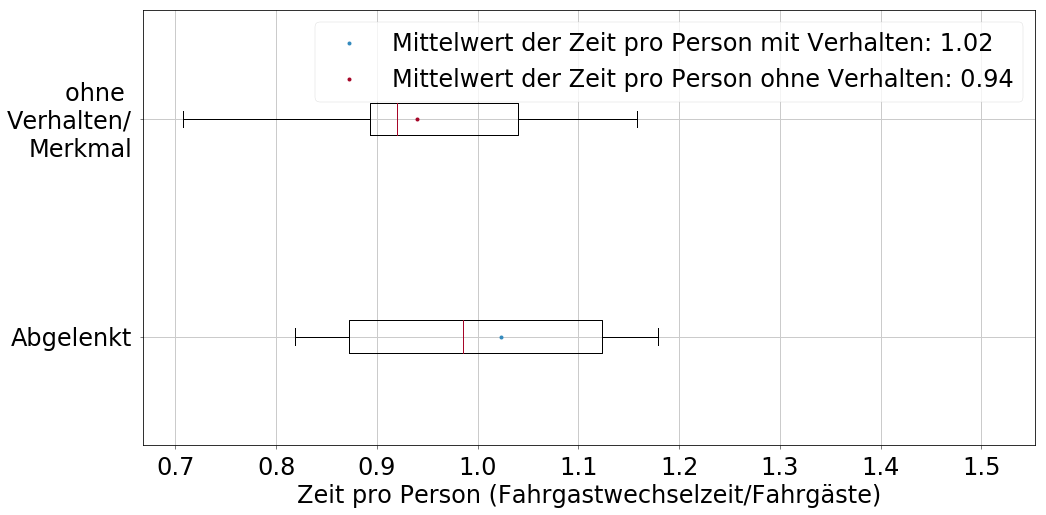
\includegraphics[width=0.8\textwidth]{pictures/data_evaluation/behavior/comp_Abgelenkt.png}
	\caption{Box-Plot für den Vergleich der Zeiten pro Person für Fahrgastwechsel in denen Personen vorkommen, die durch Gegenstände in ihrer Hand abgelenkt sind mit Fahrgastwechseln ohne abgelenkte Personen.}
	\label{fig:BoxPlotAbgelenkt}
\end{figure}
Die Signifikanz des Unterschieds ist somit deutlich geringer als vermutet. Dies ist wohl damit zu erklären, dass Personen, die durch Gegenstände in ihrer Hand vom Wechsel abgelenkt sind, sich nicht permanent mit diesem Gegenstand (\zB Handy oder Zeitung) beschäftigen. Sie sehen immer wieder auf, um zu wissen in welche Richtung sie gehen und Kollisionen sowie ein langsames Gehen zu vermeiden .

Abschließend zur Untersuchung der Merkmale, beantworte ich nun die Forschungsfrage \ref{item:Vehalten,Merkmale} "`Beeinflussen die Merkmale "`sperrig"', "`langsam"' und "`abgelenkt"' der Fahrgäste die Fahrgastwechselzeit? "'. Das Merkmal "`sperrig"' hat einen Einfluss auf die Fahrgastwechselzeit pro Person. Die Merkmale "`langsam"' und "`abgelenkt"' scheinen jedoch keinen signifikanten Einfluss auf die Zeiten des Fahrgastwechsels zu besitzen. Deshalb setze ich im Modell nur das Merkmal "`sperrig"' um. Die Merkmale "`abgelenkt"' und "`langsam"' berücksichtige ich für das Modell nicht. 

Als nächstes untersuche ich noch die Verhaltensweisen "`früher Einsteigen"' und "`im Weg Stehen"' auf ihren Einfluss auf die Zeit.\\
Bei der Verhaltensweise "`früher Einsteigen"' vermute ich, dass dieses Verhalten zu einer schnelleren Fahrgastwechselzeit pro Person führt. Diese wird nämlich, abgesehen von wenigen Ausnahmen, dann gezeigt, wenn Aussteigenden nur noch auf einer Seite der Tür in einer Reihe ausstiegen. Deshalb vermutete ich, dass die Fahrgastwechselzeit durch das frühzeitige Einsteigen sich im Gegensatz zum Warten verringert wird, oder zumindest gleichbleibt. Die Vermutung überprüfe ich durch den Vergleich der Fahrgastwechselzeiten von 12 bis 20 Personen. Auf dem Box-Plot, \figurename \ref{fig:BoxPlotFrueherEinsteigen}, ist jedoch zu sehen, dass sich die Zeit pro Person nicht verringert, sondern scheinbar sogar erhöht hat. Da diese Erhöhung jedoch nicht signifikant ist, erkennbar durch die Boxen, und ich die Veränderung so nicht erwartet habe, kann davon ausgegangen werden, dass diese Verhaltensweise keinen signifikanten zeitlichen Einfluss besitzt. Im Modell stelle ich sie jedoch trotzdem dar, um den Fahrgastwechsel besser simulieren zu können, ihr Einfluss auf die Zeit sollte bei Simulationen jedoch nicht beachtet werden.
\begin{figure}[H]
	\centering
		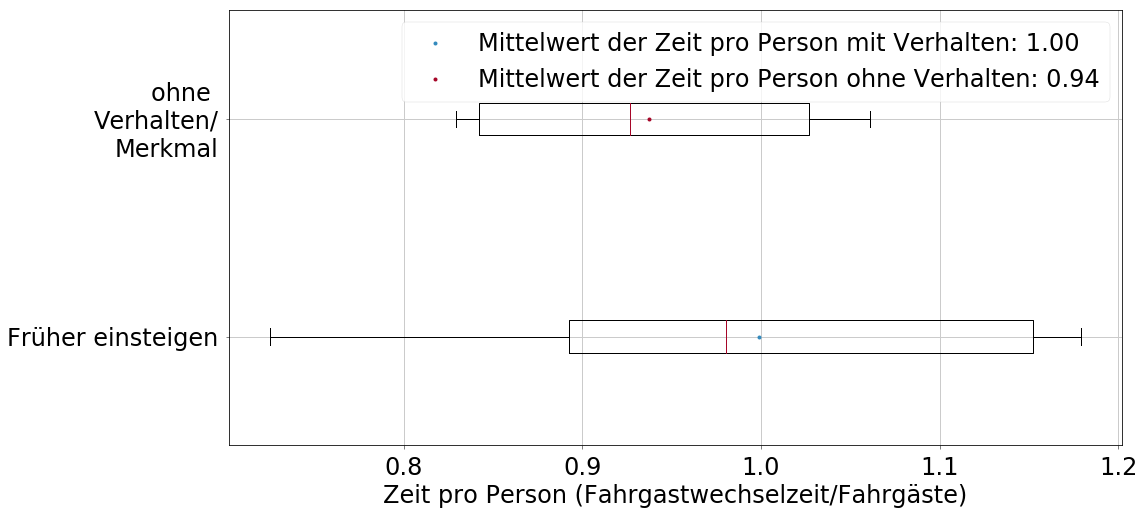
\includegraphics[width=0.8\textwidth]{pictures/data_evaluation/behavior/comp_Fruehereinsteigen.png}
	\caption{Box-Plot für den Vergleich der Zeiten pro Person für Fahrgastwechsel bei denen Personen vor Beendigung des Ausstiegsprozess Einsteigen mit, der Zeit pro Person für Fahrgastwechsel ohne Früher-Einsteiger.}
	\label{fig:BoxPlotFrueherEinsteigen}
\end{figure}
Bei der Verhaltensweise "`im Weg Stehen"' zeigt sich wie erwartet, auch eine Veränderung nach rechts, wenn die Fahrgastwechselzeiten für 19 bis 27 Personen verglichen werden. Diese Veränderung kann auf \figurename \ref{fig:BoxPlotImWeg} betrachtet werden.
\begin{figure}[H]
	\centering
		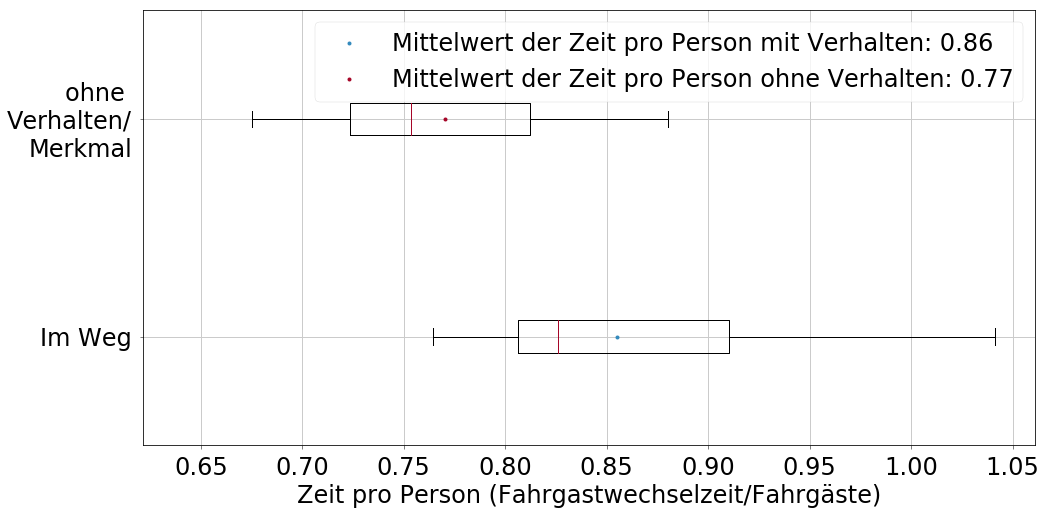
\includegraphics[width=0.8\textwidth]{pictures/data_evaluation/behavior/comp_ImWeg.png}
	\caption{Boxplot für den Vergleich der Zeiten pro Person für Personen die im Weg stehen und für andere Personen.}
	\label{fig:BoxPlotImWeg}
\end{figure}
Der Mittelwert für Fahrgastwechselzeiten pro Person mit im Weg stehenden Personen liegt mit 0.876 Sekunden über dem Wert der Zeit pro Person ohne dieses Verhalten der bei 0.806 Sekunden liegt. Zudem liegt auch das obere Quartil der Zeit mit 0.836 Sekunden pro Person unter dem Median der Fahrgastwechselzeit pro Person mit Videos bei denen Personen die "`im Weg Stehen"'. Dieser Median beträgt 0.841 Sekunden. Somit ist davon auszugehen, dass diese Verhaltensweise signifikant ist und wird deshalb in das Modell mit aufgenommen. Zudem könnte nach der Simulation gemessen werden, ob sich die Zeit der Fahrgastwechsel erhöht, wenn in einer Simulation Personen vorkamen, die im Weg standen. Der Einfluss könnte also zur Validierung des Modelles beitragen.

Auch nach der Auswertung der Verhaltensweise beantworte ich die zugehörige Forschungsfrage, \ref{item:Verhalten,Verhalten} "`Beeinflussen die Verhaltensweisen "`früher Einsteigen"' und "`Im Weg Stehen"' die Fahrgastwechselzeiten?"'. Die Verhaltensweise "`früher Einsteigen"' scheint keinen Einfluss auf die Zeit zu besitzen, während das Verhalten "`im Weg Stehen"' genau diesen zu besitzen scheint. Ich bilde jedoch beide Verhaltensweisen im Modell ab, da das Modell auf dem Verhalten der Fahrgäste und ihrem Entscheidungsprozess beruht. Deshalb ist deshalb wichtig die auffälligen Verhaltensweisen zu modellieren, um ein gutes Modell zu erhalten.

Nachdem ich den zeitlichen Einfluss der genannten Merkmale und Verhaltensweisen untersucht habe, überprüfe ich nun noch, ob es möglich ist einen Zusammenhang zwischen der Anzahl von Aussteigern und dem Auftreten von Platzmachern herzustellen.

Um den Zusammenhang, zwischen der Anzahl an Aussteigern und dem Vorkommen von Platzmachern, zu untersuchen führe ich eine logistische Regression durch. Die logistische Regression wird im Anhang in \ref{append:LogReg} noch einmal erklärt. Für den Zusammenhang in diesem Fall ist die Zielvariable das Vorkommen der Platzmacher und kodiert durch:
$$Platzmacher_i = 
	\begin{cases}
		1 & \text{falls ein Platzmacher in Fahrgastwechsel} \ i \ \text{vorkommt,} \\
		0 & \text{sonst.}
	\end{cases}$$
Um die logistische Regression zur Abschätzung des Auftretens von Platzmachern durchzuführen verwende ich das Logit-Modell:
\begin{equation}
P(Platzmacher=1) = \frac{\exp(\beta_0 + \beta_1 \cdot Anzahl \ Aussteiger)}{1+\exp(\beta_0 + \beta_1 \cdot Anzahl \ Aussteiger)}
\end{equation}
In der Bibliothek \texttt{statsmodels.discrete.discrete\_model} gibt es die Funktion \texttt{Logit}, mit der logistische Regressionen durchgeführt werden können. Diese Funktion wurde in \textsf{Jupyter Notebook} folgendermaßen aufgerufen:
\begin{lstlisting}[language=Python]
from statsmodels.discrete.discrete_model import Logit
from statsmodels.tools import add_constant

constant = add_constant(alight)
log_reg_spacemaker = Logit(cod_spacemaker, constant).fit()
\end{lstlisting}
Die Variable \texttt{alight} beschreibt die Anzahl der Aussteiger für die gefilmten Fahrgastwechsel. Die Methode \texttt{add\_constant} fügt an das \texttt{Array} der Anzahlen der Aussteiger eine Spalte mit Einsen ein. Wie ihr Name schon sagt, sorgt diese Methode dafür, dass auch eine Konstante (hier $\beta_0$) im Modell vorhanden ist. Die Variable \texttt{cod\_spacemaker} ist ein \texttt{Array}, dass die Kodierung für das Vorkommen von Platzmachern an einem Fahrgastwechsel enthält. Das Ergebnis der \texttt{fit} Methode ist ein \texttt{LogitResult} und enthält unter anderem die Schätzparameter und $p$-Werte von Hypothesentests.

Die Grafik mit der zurückgegebenen Schätzfunktion $$P(Platzmacher=1) = \frac{\exp(-2.96+0.09 \cdot Anzahl \ Aussteiger)}{1+\exp(-2.96+0.09 \cdot Anzahl \ Aussteiger)},$$
den Datenpunkten und dem Konfidenzintervall kann in \figurename \ref{fig:LogRegPM} betrachtet werden.
\begin{figure}[H]
	\centering
		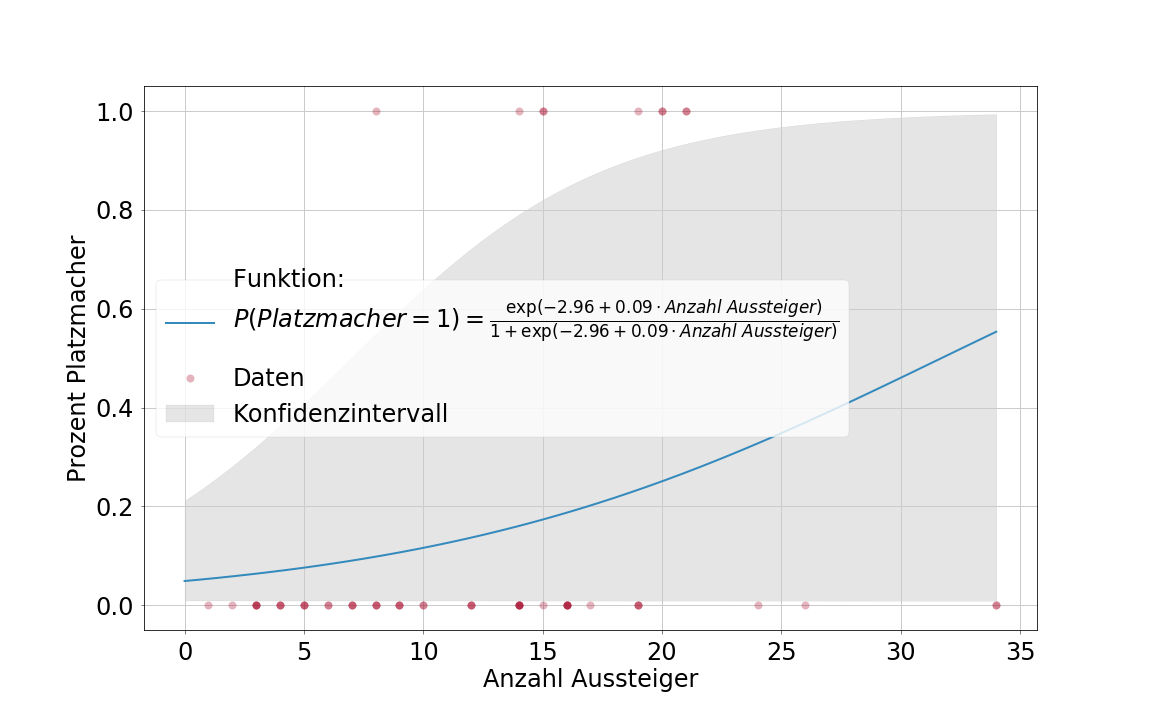
\includegraphics[width=0.8\textwidth]{pictures/data_evaluation/behavior/log_reg_spacemaker.png}
	\caption{Schätzfunktion der logistischen Regression mit der Zielvariable Platzmacher ($y$) und Kovariable Anzahl Aussteiger ($x$) mit Datenpunkten und Konfidenzintervall. Schätzfunktion: $P(y=1) = \frac{e^{-2.96+0.9 \cdot y}}{1 + e^{-2.96 + 0.9 \cdot y}}$}
	\label{fig:LogRegPM}
\end{figure}
Wie auf dem Bild zu erkennen sind die Konfidenzintervalle sehr groß und auch der $p$-Wert der t-Statistik für $\beta_1$ liegt mit $0.05$ über dem Signifikanzniveau von $0.01$. Mit meinen Daten kann also nicht modelliert werden, wann Platzmacher auftreten. Deshalb muss die Forschungsfrage \ref{item:Platzmacher} "`Gibt einen Zusammenhang zwischen der Anzahl der Aussteiger und dem Vorkommen von Platzmachern?"', mit, wohl eher nicht, beantwortet werden. \\
Es ist möglich, dass die Anzahl der Aussteiger einen gewissen Einfluss auf das Auftreten von Platzmachern hat. Mit der Anzahl der Aussteiger alleine kann jedoch nicht bestimmt werden, ob bei diesem Fahrgastwechsel ein Platzmacher auftreten wird. Ich schätze, dass der Zusammenhang weniger mit der Anzahl der Aussteiger zu tun hat, sondern eher damit, wie viele Personen sich im Wagon befinden in Kombination mit der Anzahl an Personen, die aussteigen wollen und der Position eines potenziellen Platzmacher. Eine weitere Untersuchung, die diese These überprüft, wäre mit Sicherheit interessant für das Modell.

Die Auswertungen der Verhaltensweisen und Merkmale sowie die logistische Regression des Zusammenhangs von Platzmachern und Aussteigern wurde in der Datei \textsl{Behavior.ipynb} durchgeführt die im Zusatzmaterial zu finden ist.

\section{Typen von Personen} \label{Typen}
In letzten Auswertungen beschäftige ich mich mit den Forschungsfragen \ref{item:Typen,Typen} "`Gibt es einen signifikanten Anteil an defensiven und aggressiven Personen?"' und \ref{item:Typen,Startzeiten} "`Liegen die Startzeiten der Aussteiger für die unterschiedlichen Typen in unterschiedlichen Intervallen?"'. Für die Untersuchung der Anteile von Typen werte ich die Tabelle der Typen, \tablename \ref{tab:Types} aus. Um die Forschungsfrage bezüglich der Startzeiten zu beantworten verwende ich dann die Tabelle der Startzeiten der Aussteiger \tablename \ref{tab:Startingtime}.

Im Folgenden werden die Anteile der Typen für die unterschiedlichen Prozesstypen (Einsteiger, Aussteiger und Platzmacher) in Kuchendiagrammen gezeigt. Für diese Aufteilung entscheide ich mich, da ich vermute, dass sich die Typen gegenseitig beeinflussen und durch die Art des Prozesses in der sich eine Person gerade befindet bedingt werden. Ich entschied mich dafür, dass ein Anteil signifikant ist, wenn er von mehr als 10 Prozent der Personen gezeigt wird.

Zunächst betrachte ich Anteile der Typen für Einsteiger. 
\begin{figure}[H]
	\centering
		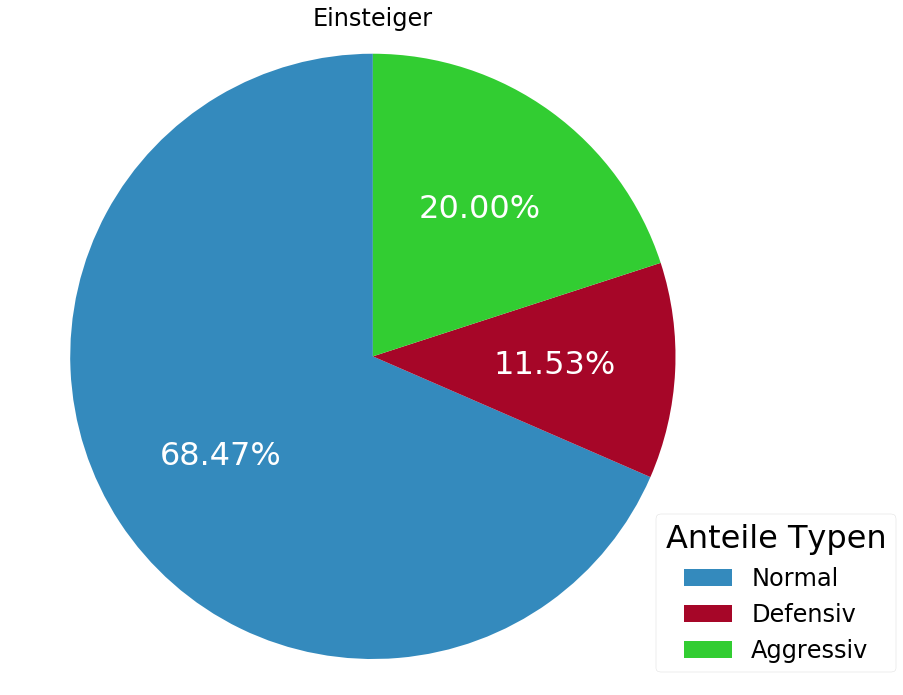
\includegraphics[width=0.6\textwidth]{pictures/data_evaluation/types/proportions_Einsteiger.png}
	\caption{Kuchendiagramm der Anteile der Typen aggressiv, defensiv und normal für den Prozesstypen Einsteiger (siehe \ref{Tabelle der Typen}).}
	\label{fig:AnteileTypenEinsteiger}
\end{figure}
Wie in \figurename \ref{fig:AnteileTypenEinsteiger} zu sehen ist, beobachtete ich am meisten normale Einsteiger, was an dem Anteil von \ca 68 \% zu erkennen ist. Mit einem Anteil von 20\% für aggressive und \ca 12\% für defensive Typen scheinen diese Typen jedoch auch signifikant zu sein. Es ist also davon auszugehen, dass ihre Modellierung zu einem besseren Modell führen würde. Die Forschungsfrage \ref{item:Typen,Typen} kann also zumindest für Einsteigende so beantwortet werden, dass ihr Anteil signifikant ist. 

In \figurename \ref{fig:AnteileTypenAussteiger} können die Anteile der Typen für Aussteiger betrachtet werden. 
\begin{figure}[H]
	\centering
		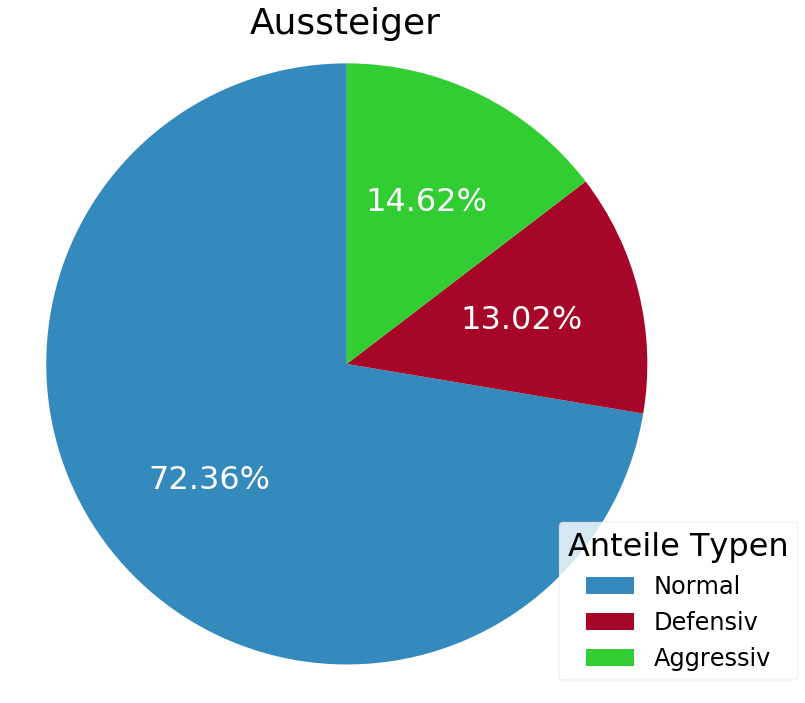
\includegraphics[width=0.6\textwidth]{pictures/data_evaluation/types/proportions_Aussteiger.png}
	\caption{Kuchendiagramm der Typen aggressiv, defensiv und normal für den Prozesstypen Aussteiger (siehe \ref{Tabelle der Typen}).}
	\label{fig:AnteileTypenAussteiger}
\end{figure}
In dem Kuchendiagramm ist zu erkennen, dass der größte Anteil an beobachteten Typen wieder der normale Typ ist. Diese Typen besitzen einen Anteil von \ca 72 \%. Jedoch gibt es auch einen signifikanten Anteil an defensiven und aggressiven Typen, wobei defensive einen Anteil von 13 \% und aggressive einen Anteil von \ca 15 \% ausmachen. Für Aussteiger ist die Frage \ref{item:Typen,Typen} also auch mit ja zu beantworten. Da es hier signifikante Anteile für die Typen defensiv und aggressiv gibt, wäre es gut auch die Aussteiger im Modell in aggressive, defensive und normale Typen zu unterteilen.

Als nächstes werte ich nun noch die Anteile der Platzmacher aus.
\begin{figure}[H]
	\centering
		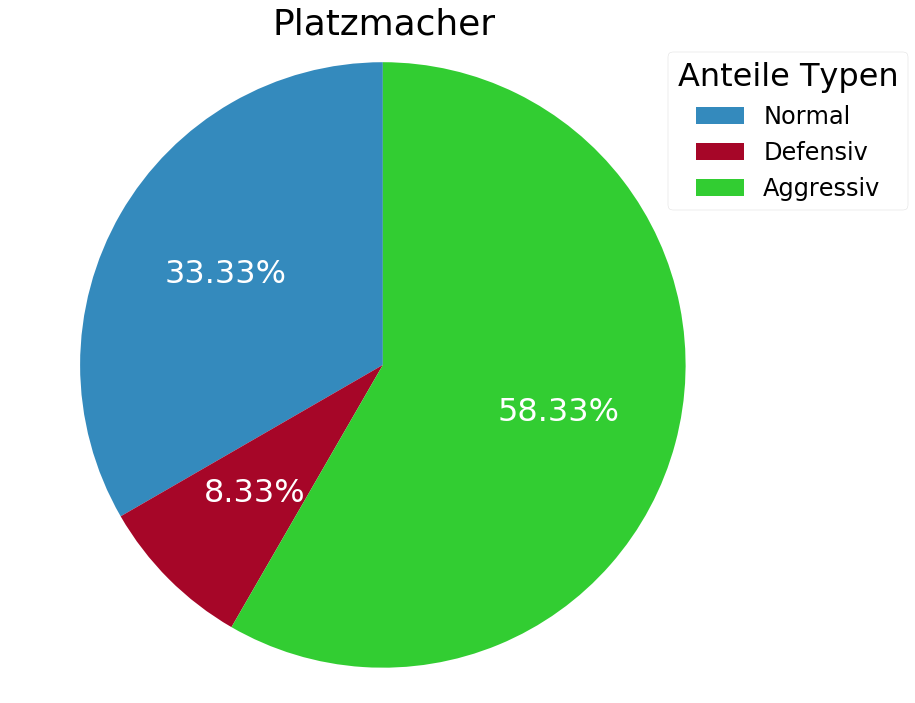
\includegraphics[width=0.7\textwidth]{pictures/data_evaluation/types/proportions_Platzmacher.png}
	\caption{Kuchendiagramm der Typen aggressiv, defensiv und normal für den Prozesstypen Platzmacher (siehe \ref{Tabelle der Typen}).}
	\label{fig:AnteileTypenPlatzmacher}
\end{figure}
In \figurename \ref{fig:AnteileTypenPlatzmacher} ist nun zuletzt das Kuchendiagramm der Anteile von Typen der Platzmacher zu sehen. Bei den Platzmachern überwiegen, im Gegensatz zu den anderen Prozesstypen, die aggressiven Typen mit über 50\% (53.85\%). Der Anteil der normalen Typen macht mit \ca 38\%  auch einen großen Anteil aus. Es gibt jedoch auch einen Anteil an defensiven Platzmacher. Mit 7.69\% scheinen diese jedoch nicht signifikant zu sein. Da der defensive Typ für Aussteiger und Einsteiger jedoch in das Modell mit aufgenommen werden soll, soll dieser auch für Platzmacher definiert werden, um das Modell konsistent zu halten. Es ist jedoch auch anzumerken, dass der Anteil von 7.69\% wahrscheinlich nur durch die geringe Anzahl an aufgenommenen Platzmachern zustande gekommen ist. Im Material wurde nur ein einziger defensiver Platzmacher gesehen, da ich jedoch nur sehr wenige Platzmacher beobachtet habe, ist nicht festzustellen, ob der Anteil sich verringern würde, wenn mehr Platzmacher beobachtet werden. Da die Platzmacher sowohl ein- als auch aussteigen, wird die Forschungsfrage auch für diesen Prozesstypen mit Ja beantwortet. 

Im Modell wird der Entscheidungsprozess der Personen dargestellt, hierbei passe ich die Ein- und Aussteiger sowie Platzmacher zudem für defensive, aggressive und normale an, da sich der Entscheidungsprozess für diese Typen unterscheidet. Dies kann am Beispiel der ersten Person, die aus dem Wagon aussteigt, erkannt werden. Während aggressive schon kurz nach der Türöffnung aussteigen, warten defensive bis diese komplett geöffnet ist und normale Personen bis die Tür etwas weiter geöffnet ist. Es ist jedoch schwierig in einer Simulation zu beschreiben, wie weit eine Tür geöffnet ist. Deshalb untersuchte ich, ob für die Typen aggressiv, defensiv und normal unterschiedliche Intervalle für die Startzeiten gefunden werden können. Mit den Intervallen wird dann modelliert, wann Aussteiger mit dem Aussteigen beginnen. Diese Untersuchung führe ich im nächsten Abschnitt, Abschnitt \ref{Startzeiten} durch.

Die Kuchendiagramme der Anteile von Typen für die unterschiedlichen Prozesstypen wurden in der Datei \textsl{TypesOfPeople.ipynb} mit \texttt{Python} erstellt.

\subsection{Startzeiten der Aussteiger für die Typen} \label{Startzeiten}
Nachdem ich im Vorangegangen erklärt habe, warum es interessant ist Aussteiger in unterschiedlichen Typen einzuteilen um modellieren zu können wann diese mit dem aussteigen beginnen, beantworte ich nun die aufgekommene Frage: "`Liegen die Startzeiten der Aussteiger für die unterschiedlichen Typen in unterschiedlichen Intervallen?"'\\
Zu diesem Zweck trug ich in der Tabelle der Startzeiten, \tablename \ref{tab:Startingtime}, die Zeiten aus den Videos ein, die verstreicht bevor die erste Person aus dem Zug aussteigt. Hier gab ich zudem in einer weiteren Spalte der Tabelle an, welchem Typ der erste Aussteiger in diesem Video zuzuordnen ist. 

Mit den Daten aus der Tabelle erstellte ich Box-Plots für die Startzeiten der Typen, die in \figurename \ref{fig:BoxPlotStartingTime} betrachtet werden können.
\begin{figure}[H]
	\centering
		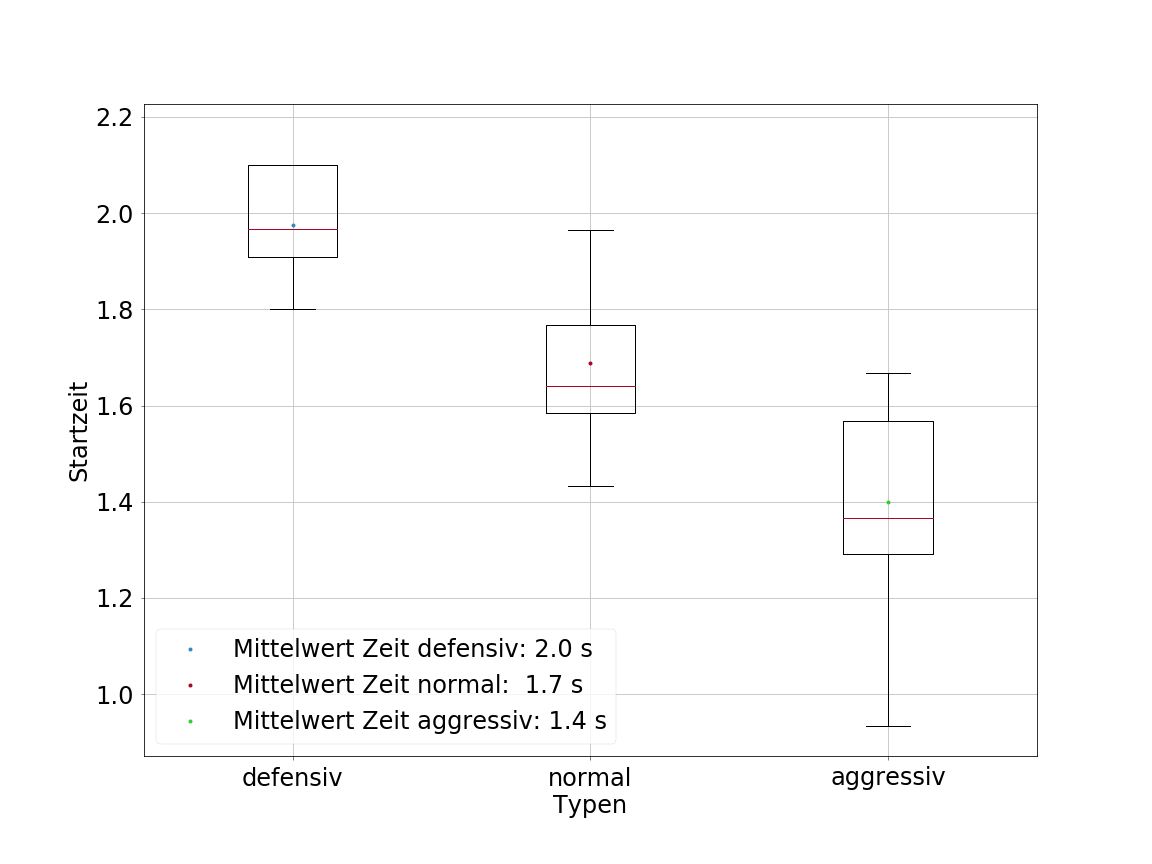
\includegraphics[width=1.0\textwidth]{pictures/data_evaluation/types/starting_time/starting_times.png}
	\caption{Box-Plots der Startzeiten für die unterschiedlichen Typen aggressiv, defensiv und normal von Aussteigern.}
	\label{fig:BoxPlotStartingTime}
\end{figure}
Auf diesem Plot ist zu erkennen, dass sich die Startzeiten der Aussteiger für die unterschiedlichen Typen defensiv, aggressiv und normale unterscheidet, wie ich bei der Beobachtung vermutet habe. Während die defensiven mit 2.0 Sekunden im Mittel am längsten warten, ergeben die Mittelwerte für normale und aggressive Typen das diese im Mittel 1.7 \bzw 1.4 Sekunden warten, bevor sie mit dem Aussteigen anfangen. Für die Startzeit soll jedoch kein fester Wert verwendet werden, sondern jeweils ein Zeitraum für defensive, aggressive und normale gewählt werden. Hierfür untersuchte ich die Histogramme der Startzeiten für die Typen. Da jedoch nur sehr wenige Daten vorhanden sind, konnten diese nicht auf ihre Verteilung untersucht werden. Deshalb entschied ich, dass der Zeitraum durch die Quartile festgelegt wird. Für die untere Schranke des Startzeitraums wählte ich jeweils das 25\%-Quantil, für die obere das 75\%-Quantil, der Startzeiten für den entsprechenden Typ. \\ 
Damit ergibt sich für die Intervalle: \\
Startzeiten Intervall für den Typ "`normal"' $= [1.6, 1.8]$ Sekunden. \\
Startzeiten Intervall für den Typ "`aggressiv"' $= [1.3, 1.6]$ Sekunden. \\
Startzeiten Intervall für den Typ "`defensiv"'$= [1.9, 2.1]$ Sekunden. 

Es kann also gesagt werden, dass ein Zeitraum für die Startzeiten für verschiedene Typen von Aussteigern festgelegt werden konnte. Damit ist auch die Forschungsfrage \ref{item:Typen,Startzeiten} beantwortet worden. Die definierten Intervalle sollen später im Modell für den Entscheidungsprozess der Aussteiger verwendet werden.
